\documentclass[
	%parspace, % Add vertical space between paragraphs
	%noindent, % No indentation of first lines in each paragraph
	%nohyp, % No hyphenation of words
	%twoside, % Double sided format
	%draft, % Quicker draft compilation without rendering images
	%final, % Set final to hide todos
]{elteikthesis}[2023/04/10]

% The minted package is also supported for source highlighting
% See elteikthesis_minted.tex for example
%\usepackage[newfloat]{minted}
\usepackage{amssymb}
\usepackage{amsmath}
\usepackage{physics}

\usepackage{xparse}
\NewDocumentCommand{\codeword}{v}{%
	\texttt{#1}%
}

% Document's metadata
\title{Parametrikus felületek távolságmezőjének generálása és megjelenítése} % title
\date{2023} % year of defense

% Author's metadata
\author{Szente Péter}
\degree{programtervező informatikus BSc}

% Superivsor(s)' metadata
\supervisor{Bán Róbert} % internal supervisor's name
\affiliation{doktorandusz} % internal supervisor's affiliation
%\extsupervisor{Külső Kornél} % external supervisor's name
%\extaffiliation{informatikai igazgató} % external supervisor's affiliation

% University's metadata
\university{Eötvös Loránd Tudományegyetem} % university's name
\faculty{Informatikai Kar} % faculty's name
\department{Numerikus Analízis Tanszék} % department's name
\city{Budapest} % city
\logo{elte_cimer_szines} % logo

% Add bibliography file
\addbibresource{elteikthesis.bib}

% The document
\begin{document}

% Set document language
\documentlang{hungarian}
%\documentlang{english}

% List of todos (not in the final document)
%\listoftodos[\todolabel]

% Title page (mandatory)
\maketitle
% Topic declaration page (mandatory) - can also be attached instead
%\includepdf{temabejelento.pdf}

% Table of contents (mandatory)
\tableofcontents
\cleardoublepage

% Main content
\chapter{Bevezetés}
\label{ch:intro}

\section{Témaválasztás és feladatleírás}

A számítógépes modellezés egyik meghatározó eszköze a testek felületének különböző parametrikus felületekkel való leírása. Egyre szélesebb körben elterjedő implicit felületreprezentáció az előjeles távolságfüggvények és diszkretizált változatuk, a távolságmezők. A távolságmezővel reprezentált felület egy speciális sugárkövető eljárással, a sphere tracinggel jeleníthető meg.

A szakdolgozat célja parametrikus felületekkel ábrázolt objektumok távolságmezőjének generálására GPU segítségével. A létrejövő távolságmezők megjeleníthetők GPU-val gyorsított módon, az említett sphere tracing módszerrel. Ezt a módszert összehasonlítom a parametrikus felület háromszögekkel tesszellált megjelenítésével.

A távolságmezőt felhasználom még geometriai lekérdezések elvégzésére, mint a felületi normális meghatározása, ami a felület árnyalásához elengedhetetlen. Meghatározhatók még láthatósági viszonyok, melyet vetett árnyékok számításánál használok.

A készített programmal kétdimenziós függvények grafikonjai és Bézier-felületek jeleníthetők meg. A Bézier-felületekre azért esett a választás, mert a kontrollpont-hálójukon keresztül intuitívan manipulálhatók és a folytonosság megtartása mellett összeilleszthetők, így különösen alkalmasak felületek modellezésére. Harmadfokú Bézier-felületek távolságmezőjének generálására speciális algoritmust is adok, melyet összehasonlítok a korábban tárgyalt módszerekkel.

\section{Szakirodalmi áttekintés}

A téma \citeauthor{Hart1996} cikkével \cite{Hart1996} kezdődik, melyben bemutatja, hogyan használható a sphere trace algoritmus felületek megjelenítésére. A módszer a sugárkövetést gyorsítja fel azzal, hogy a felülettől vett távolsággal lép a sugáron. Ez különösen a felülettől távol eredményez gyorsítást. A módszer előfeltétele, hogy a távolságfüggvényt viszonylag gyorsan ki tudjuk számítani. Ez könnyen megtehető egyszerűbb testek esetében. A módszert általában a GPU pixel shaderében implementálják, így a teljes színtér eltárolható GPU kódként. Emiatt a Demoscene-ekben nagyon sok példát látunk rá. Ilyeneket gyűjt össze például a Shadertoy weboldal.

Ha a felületek távolságfüggvénye nehezen számítható, vagy a jelenet túl összetett, akkor közelítésekre lehet szükség. Ha a távolságfüggvény becslés nem elég jó, akkor a sugárkövetés lelassul. Az alap sugárkövető algoritmus felgyorsítására több módszer is született. \cite{Keinert2014EnhancedST,BálintValasekAccST,QuadricTrace,RobBan} A sugárkövetés gyorsítható, ha a távolságfüggvényt egy diszkrét rácson kiértékeljük, és az eredményt letároljuk. Ennek a műveletnek nem kell valós idejűnek lennie, minden objektumra előszámítható. A távolságmezőből a távolságfüggvény becslését úgy kapjuk, hogy a szomszédos 8 pontot trilineárisan interpoláljuk. Ha a távolságmezőben pontos értékek vannak, akkor a 8 távolság által reprezentált harmadfokú felület pontosan rekonstruálható. \cite{Hansson-Soderlund2022SDF}



\cleardoublepage

% ------------------------------------------------------
\chapter{Felhasználói dokumentáció}
\label{ch:user}
% ------------------------------------------------------




% ------------------------------------------------------
\chapter{Elméleti háttér}
% ------------------------------------------------------

A sugárkövetéssel történő képszintézisről részletes összefoglaló olvasható Bálint Csaba OTDK dolgozatában \cite[11-16. o.]{BalintCsaba}, így azt itt nem részletezem.

\section{Sphere tracing}

Adott egy $d:\mathbb{R}^n\rightarrow\mathbb{R}$ előjeles távolságfüggvény, mely minden bemenetre a pont a felület határától vett előjeles távolságát adja. Ez az érték a felület által határolt térrész belsejében negatív, kívül pedig pozitív. Formálisan $d$ akkor távolságfüggvény, ha az alábbi teljesül \cite{Hart1996}:
$$f(p) = d(p, f^{-1}(0)) (p \in \mathbb{R}^n)$$

A sugárkövetés során adott egy kiinduló pont és egy sugárirány. A cél a félegyenes-felület metszéspont megtalálása. Míg a sugármetszés egyszerűbb matematikai objektumok esetén (pl. gömb, sík) analitikusan elvégezhető, bonyolultabb testek esetén csak óvatosabban közelíthetünk a felülethez a sugáron. (Ray Marching\cite{RayMarching})

A sphere trace algoritmusról Hart cikkében \cite{Hart1996} részletesen olvashatunk. Röviden összefoglalva a sphere trace egy sugárkövető algoritmus, mely minden lépésben kiértékeli a távolságfüggvényt. Tudjuk, hogy a távolságfüggvénnyel megegyező méretű üres tér van a pont körül, hiszen az a felülethez vett távolság minimumát, vagy annak \emph{alsó közelítését} adja. Ekkor a távolsággal megegyező méretűt léphetünk a sugár mentén. A sugárkövetés a felület közelében lelassul. Ha a távolság epszilonnál kisebb, vagy fix lépésszám után leállítjuk az iterációt.  


\section{Előjeles távolságfüggvények}


\subsection{Egyszerűbb alakzatok}
Inigo Quilez oldalán \cite{QuilezDistanceFunctions} felsorolja sok egyszerűbb alakzat analitikus távolságfüggvényét. Például egy $o$ középpontú és $r$ sugarú gömb előjeles távolságfüggvénye:
$$ d_{g}(p) = \norm{p-o}_2 - r $$
A weboldalon további testek távolságfüggvényei is láthatók. Ezekből aztán könnyen építhetünk színteret az alábbi tömörtest-modellezésben is használt műveletekkel: (Legyen az $A$ testtől vett előjeles távolságfüggvény $d_A$, a $B$ testtől vett pedig $d_B$)

\begin{itemize}
	\item Mivel a távolságfüggvény a legközelebbi távolságot adja, két test uniója a távolságfüggvények minimuma. $d(A\cup B) = min(d_A, d_B)$
	\item  Egy test ,,kifordítható'', ha a távolságfüggvény $-1$-szeresét vesszük $d\left(\overline{A}\right) = -d_A$.
	\item Két test metszete a távolságfüggvények maximuma, hiszen addig haladhatunk a sugár mentén, amíg mindkét alakzatot el nem találjuk. $d(A\cap B) = max(d_A, d_B)$
	\item Kivonást is elvégezhetünk, ha a test és a kifordított test metszetét vesszük. $d(A\backslash B) = max(d_A,-d_B)$ 
\end{itemize}

Elvégezhetők még a testeken transzformációk, ami általában a mintavételezési pontra alkalmazott inverz-transzformációval történik. Ilyenek például a nagyítás, nyújtás, lekerekítés, forgatás, kétdimenziós alakzat kiterjesztése hasábbá vagy forgástestté.

Különösen érdekesek a tükrözés, ami az abszolút érték függvénnyel elvégezhető, illetve az alakzat véges és végtelen ismétlése, melyet a koordinátára alkalmazott moduló operátorral lehet elérni. \cite{QuilezDistanceFunctions}


\subsection{Parametrikus felületek távolságfüggvénye}

Háromdimenziós euklideszi térben parametrikus egyenlettel megadott felületeket hívjuk így. $f:\mathbb{R}^2\rightarrow\mathbb{R}^3$ Azért felület, mert a vektor-értékű függvény értelmezési tartomány beli pontjaihoz háromdimenziós pontokat rendelünk. Modellezéskor így a test felszínét adjuk meg.  Például a tórusz parametrikus egyenlete:
$$ f(u,v) = \begin{pmatrix} 
	r\cdot sin(v) \\ 
	(R+r\cdot cos(v))\cdot sin(u) \\ 
	(R+r\cdot cos(v))\cdot cos(u)
\end{pmatrix} $$
Ahol $r$ a generáló kör sugara, $R$ pedig a forgástengely és a kör középpontjának távolsága. $u$ és $v$ szögek, így $u,v\in[0,2\pi]$  
Parametrikus egyenlettel megadhatók függvények grafikonjai is. Legyen $h(u,v)$ a függvény, ekkor a grafikon parametrikus egyenlete:
$$ f(u,v) = (u,v,h(u,v)) $$
\begin{figure}[H]
	\centering
	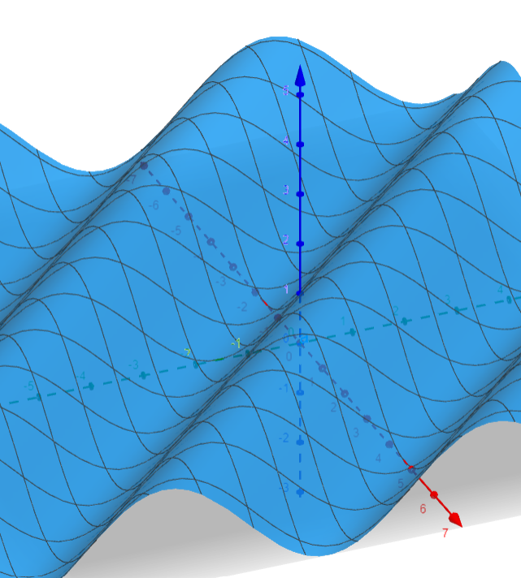
\includegraphics[width=0.3\textwidth]{sinuv}
	\caption{$h(u,v) = sin(u+v)+1$ grafikon a GeoGebra alkalmazásban.}
\end{figure}

Ezen felületek távolságfüggvénye analitikusan sok esetben nem meghatározható. Vegyünk egy kétdimenziós példát, az $y = sin(x)$ függvényt és egy $(e,f)$ mintavételezési pontot, amihez a legközelebbi pontot keressük a felületen. ekkor a minimalizálandó függvény: 
$$ d(x) = \sqrt{(x-e)^2+(sin(x)-f)^2} $$
A gyök függvény szigorú monotonitása miatt vizsgáljuk $d^2$ minimumát. Az elsőrendű szükséges feltétel: 
$$ cos(x)\cdot(sin(x)-f)+x-e = 0 $$ 
Ezt csak néhány speciális esetben tudjuk analitikusan megoldani.

Polinomokkal sem boldogulunk könnyen analitikus módszerekkel. Például ha a polinom fokszáma harmadfokú, akkor a négyzetre emelés és deriválás után egy ötödfokú polinom gyökeit kellene meghatározni. Erre már nem létezik megoldóképlet. Ez az eset előkerül a dolgozatomban a Bezier felületek tárgyalásánál.


\section{Bézier görbék}

Ennek a résznek alapul G. Farin: Curves and Surfaces for CAGD című könyve szolgált. \cite{farin2002curves} A de Casteljau-algoritmusról és Bézier-görbékről a könyv 45-47., a Bernstein-polinomokról a könyv 57. oldalán olvashatunk. Ezeket itt nem részletezem, csak a szükséges tételeket mutatom be. 

\subsection{Bernstein-alak}
Az $i$-edik $n$-edfokú Bernstein-polinom alakja:
$$ B^n_i(t) = \binom{n}{i}t^i(1-t)^{n-i} $$
Legyenek egy $n$-edfokú Bézier-görbe kontrollpontjai $b_0,b_2,\dots,b_n$ Ekkor a görbe felírható Bernstein-bázisban:
$$ b(t) = \sum_{i=0}^n b_i B^n_i(t) $$
Ezt a görbe Bernstein-alakjának is nevezik

\subsection{Végpont interpoláció}
A Bernstein-polinomok tulajdonságaiból adódik, hogy a görbe a végpontjaiban egyenlő a szélső kontrollpontokkal, azaz interpolál.

\subsection{Pszeudolokális kontroll}
A legfontosabb tulajdonsága ezen görbéknek, hogy egy kontrollpont megváltoztatása csak annak környezetét változtatja meg jelentősen. Ennek oka, hogy $B^n_i(t)$-nek egyetlen maximuma van, a $t = i/n$ helyen. \cite[62. o.]{farin2002curves}

A végpont interpoláció és a pszeudolokális kontroll miatt a görbe különösen alkalmas számítógépes modellezésre, mivel a felület a kontrollponthálójával intuitívan manipulálható.

\subsection{Derivált}
A görbe deriváltja: \cite[63. o.]{farin2002curves}
$$ b'(t) = n\sum_{i=0}^{n-1} \Delta b_i B^{n-1}_i(t) $$
Ahol $\Delta b_i = b_{i+1} - b_i$ ($\Delta$ a jobboldali differenciaoperátor.)



\section{Bézier-felületek}

\subsection{Bilineáris interpoláció}
Farin a Bézier felületeket a tenzor szorzat felületek bevezetéseként írja le. Egy egyik irámyban $m$, másik irányban $n$-edfokú felületet $(m+1)\cross(n+1)$ kontrollpont definiál. A felület pontjai kiszámíthatók a kontrollpontháló ismételt bilineáris interpolációjával. Ezt a felület pontbeli kiértékelésének nevezzük.

\begin{figure}[H]
	\centering
	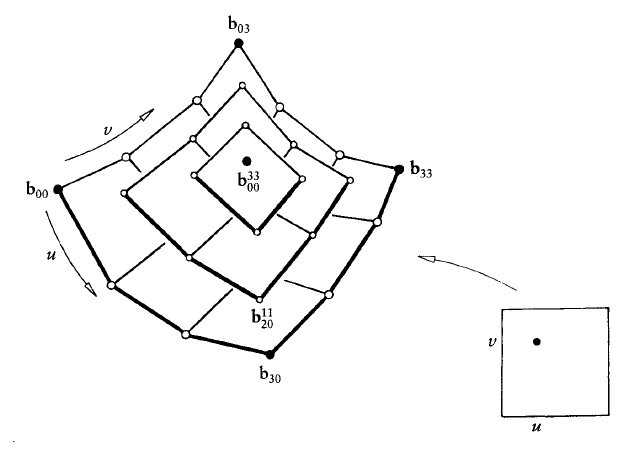
\includegraphics[width=0.5\textwidth]{Farin_bilinear}
	\caption{Bézier-felület kiértékelése \cite[248. o.]{farin2002curves}}
\end{figure}

\subsection{Bernstein-alak}
A végeredmény szempontjából lényegtelen, hogy az interpolációkat milyen sorrendben végezzük. Például kiértékelhetjük a kontrollponthálót az egyik paraméter szerint, majd az így keletkezett kontrollpontok által definiált Bézier-görbét a másik paraméter szerint. \cite[251. o.]{farin2002curves} A felület Bernstein-alakja:
$$ b^{m,n}(u,v) = \sum_{i=0}^m \sum_{j=0}^n b_{i,j}\, B^m_i(u) B^n_j(v) $$

\subsection{Parciális deriváltak}
A könnyebb leírás érdekében bevezetjük a parciális differenciaoperátort. Ennek szabályai: $\Delta^{1,0}b_{i,j} = b_{i+1,j} - b_{i,j}$ és  $\Delta^{0,1}b_{i,j} = b_{i,j+1} - b_{i,j}$

A parciális deriváltat a Bézier-görbe deriváltjára vezetjük vissza:
$$ \partial_u b^{m,n}(u,v) = \sum_{j=0}^n \left[\partial_u \sum_{i=0}^m b_{i,j} B^m_i(u) \right] B^n_j(v) $$
$$ \partial_u b^{m,n}(u,v) = m\sum_{j=0}^n \sum_{i=0}^{m-1} \Delta^{1,0} b_{i,j} B^{m-1}_i(u)  B^n_j(v) $$
A másik parciális derivált hasonlóan meghatározható:
$$ \partial_v b^{m,n}(u,v) = n\sum_{j=0}^{n-1} \sum_{i=0}^m \Delta^{0,1} b_{i,j} B^m_i(u)  B^{n-1}_j(v) $$
Magasabbrendű deriváltakat a dolgozatban nem használtam, így azokat itt nem tárgyalom. Az általános alak szintén megtalálható Farin könyvében.



\section{Legközelebbi pont meghatározása}

A legközelebbi pont meghatározása nem egyszerű feladat. Egyszerűsítésként egy $b(x,y)$ függvény grafikonjára próbáljuk meg meghatározni. Ezen belül is vegyünk egy harmadfokú Bézier-felületet.

\subsection{Merőlegesség feltétel}
A legközelebbi pont szükséges feltétele: Az $E$ mintavételezési pontból a felületi pontba húzott egyenes merőleges mindkét parciális deriváltra. Egyik irányra felírva:
$$ r(x,y) = (x,y,b(x,y)) $$
$$ \frac{dr}{dx} = (1,0,b_x(x,y)) $$
Ahol $b_x$ az első koordináta szerinti parciális derivált. A mintavételezési pont legyen az origó. Ezt megtehetjük, hiszen a felületet átparaméterezhető úgy, hogy a mintavételezési pont az origóba essen. Ha két vektor merőleges, a skalárszorzatuk $0$.
$$ 0 = \left\langle r, \frac{dr}{dx} \right\rangle = \begin{pmatrix} 1 $ 0 $ b_x(x,y) \end{pmatrix} \cdot \begin{pmatrix} x \\ y \\ b(x,y)\end{pmatrix} = x + b_x(x,y)b(x,y) $$
$x$ szerint parciálisan integrálva: 
$$ f(y) = x^2/2 + b(x,y)^2 $$
$$ x=0 \rightarrow f(y) = b(0,y)^2 $$
$$ b(0,y)^2 = x^2/2 + b(x,y)^2 $$
A feltétel barátságos alakja ellenére a mi esetünkben (harmadfokú Bézier) ez egy ötödfokú kétismeretlenes egyenlet tetszőleges együtthatókkal. 

Látjuk, hogy ez a megközelítés nem vezet eredményre. Ugyanezt az egyenletet kapjuk, ha a szükséges feltételt a felületi normális segítségével írjuk fel. Ezt itt nem részletezem. Az algoritmusok résznél a problémára több közelítési módszert is bemutatok.

% ------------------------------------------------------
\chapter{Algoritmusok}
% ------------------------------------------------------

\section{Tesszelláció}

A legelső megjelenítési mód a felület háromszögekkel való közelítése. A Tesszelláció vagy háromszögelés során a cél úgy lefedni háromszögekkel a felületet, hogy annak részletei ne vesszenek el. Ez egyben a leggyakrabban használt modellezési módszer is. A videókártyák hardveresen támogatják háromszögek raszterizációját, így ez a módszer nagyon gyors. A többi módszer helyességét a háromszögekkel tesszellált közelítéssel fogom ellenőrizni. Ha függvények grafikonjait háromszögeljük, általában egyenletes felosztást veszünk a parmétertérben. A függvényértéket a harmadik koordináta reprezentálja.

\begin{figure}[H]
	\centering
	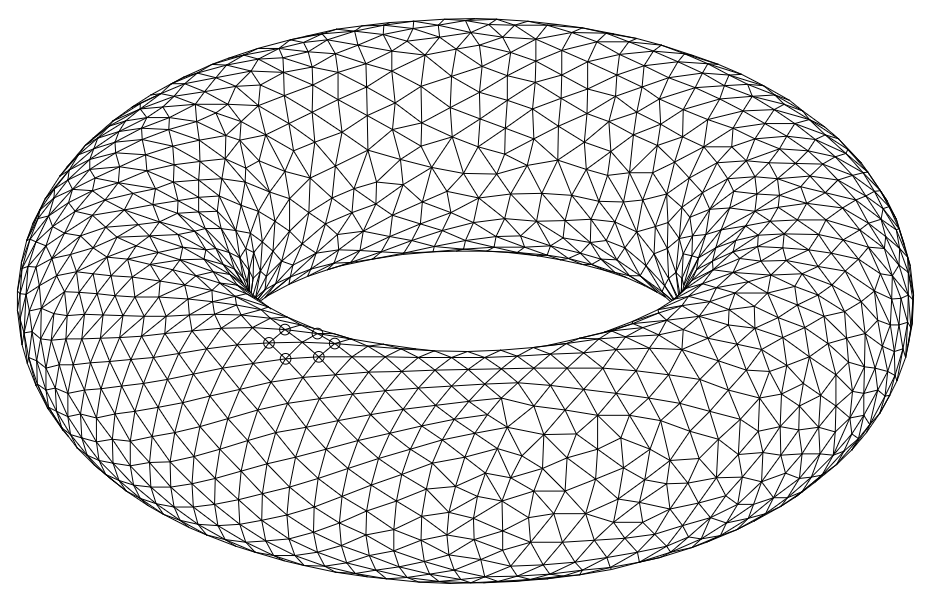
\includegraphics[width=0.4\textwidth]{tess_torus}
	\hspace{5pt}
	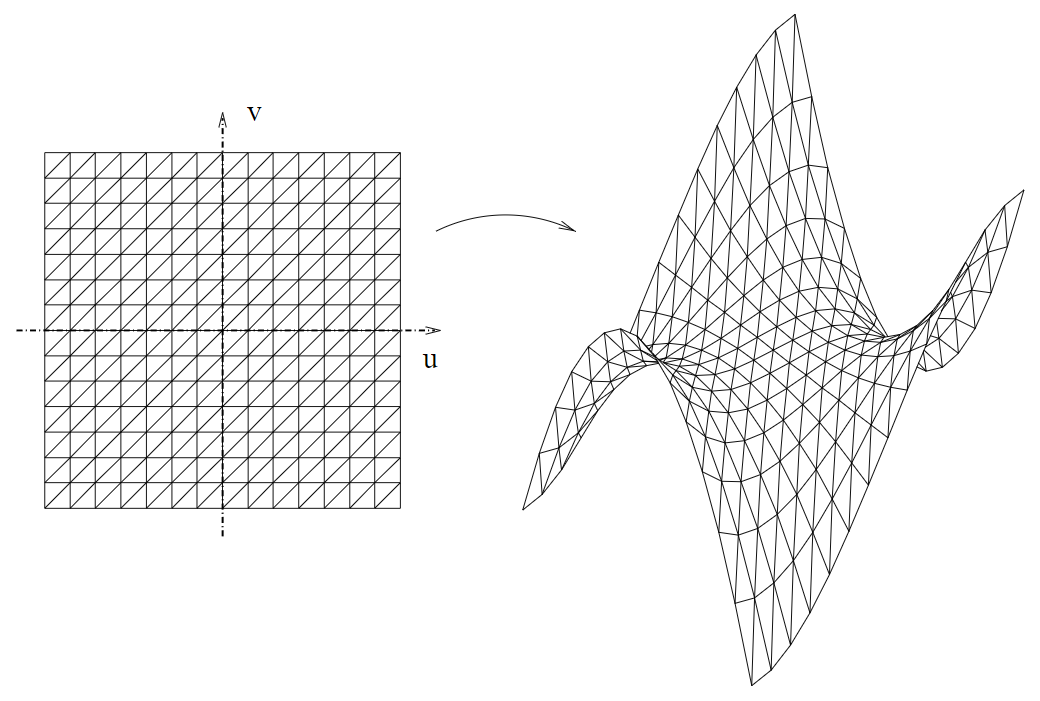
\includegraphics[width=0.4\textwidth]{tess_graph.png}
	\caption{Tórusz és függvénygrafikon háromszögelése. Forrás: \href{https://www.wikiwand.com/en/Surface_triangulation}{wikiwand.com}}
\end{figure}


\section{Sugárkövetés motivációja}

A sugárkövetés mindenképpen költségesebb művelet, mint a raszterizáció, hiszen visszaverődéseket, törést és árnyéksugarakat is számítunk a jobb eredmény érdekében. Ha a fotorealisztikus eredmény a cél, akkor viszont mindenképpen sugárkövetést használunk és a cél az extra számítási költségek csökkentése, a sugárkövetés felgyorsítása. 

\begin{figure}[H]
	\centering
	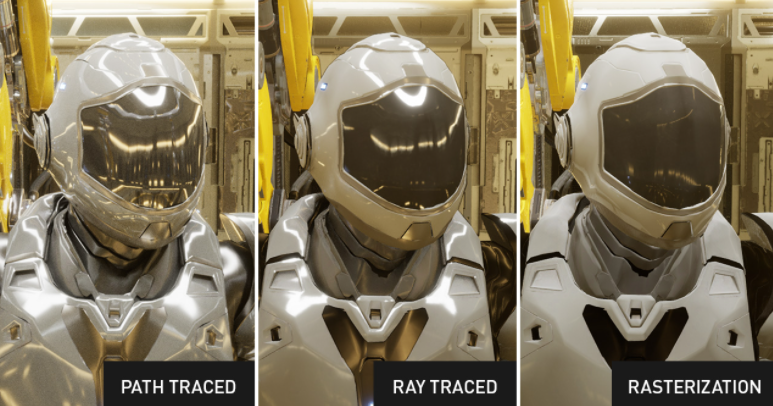
\includegraphics[width=0.7\textwidth]{pt-rt-raster}
	\caption{Megjelenítési módok összehasonlítása. Forrás: \href{https://blogs.nvidia.com/blog/2022/03/23/what-is-path-tracing/}{blogs.nvidia.com}}
\end{figure}


\section{Fénymodell}

Fénymodellnek egy egyszerű Blinn-Phong árnyalást használtam \cite{Blinn1977} árnyéksugarakkal. Az árnyéksugár számítás ugyanazt az algoritmust használja, mint a sugárkövetés. Ha elmetsszük a felületet a felületi pontból a (pont)fényforrás felé indított sugárral, akkor a felületi pont árnyékban van.

Fontos megemlíteni, hogy a távolságfüggvények segítségével puha árnyékszámító algoritmus is adható. \cite{AreaLights}


\section{Távolságfüggvény rács számítása}

A távolságfüggvényt egy diszkrét rácson értékelem ki, melyet egy háromdimenziós textúrában tárolok. Mivel csak a mintavételezési pont változik, maga a kiértékelendő (vagy meghatározandó) távolságfüggvény nem, így ki tudom használni a GPU masszívan párhuzamos architektúráját. A textúrát saját GPU compute shaderek segítségével számítom ki. A számítás elvégzésére később több módszert is mutatok. 

Fontos megjegyezni, hogy ennek a műveletnek nem kell valós idejűnek lennie. A program indításakor a textúra több frame alatt kiszámítható. Ezután elég a textúrát a fragment shader számára feltölteni a GPU-ra a sugárkövetés előtt.


\section{Sugárkövetés távolságmezőn}

A sugárkövetés során adott a kiinduló pont $P$, és a sugár iránya $d$. Emellett adott egy $F$ függvény, mely az előbb részletezett textúra olvasást és bilineáris interpolációt elvégzi, majd visszaadja a távolságfüggvény becslését. A távolságfüggvény rácsból az értékeket a textúra bilineáris interpolációjával nyerem ki. Ez a fajta textúra mintavételezés egy hardveresen támogatott művelet a GPU-n. Az alábbi függvény a kiindulási pont és a sugár felülettel vett első metszéspontjának távolságát adja meg.

\begin{algorithm}[H]
	\caption{Sugárkövetés távolságmezőn}
	\label{alg:ibb}
	\textbf{\underline{Funct}} DSFBoxTrace($P,d,F$)
	\begin{algorithmic}[1] % sorszámok megjelenítése minden n. sor előtt, most n = 1
		\If{$P$ a dobozon kívül van}
		\State{\textbf{return} $-1$} \Comment{Távolság nem definiált}
		\EndIf
		\If{$F(P) \leq 0$}
		\State{\textbf{return} $0$} \Comment{A doboz oldalán már a felületben vagyunk}
		\EndIf
		\State{$depth := 0$}
		\For{$i \gets 1$ to maxSteps} \Comment{Maximum lépésszám}                    
		\State{$dist := F(P + depth * d)$}
		\If{$abs(dist) < \varepsilon$}
		\State{\textbf{return} $depth$} \Comment{Eltaláltuk a felületet}
		\EndIf
		\State{$depth\; +\! = dist$}
		\State{$currPos := P + depth * d$}
		\If{$currPos$ a dobozon kívül van}
		\State \textbf{return} $-1$; \Comment{Távolság nem definiált, nincs metszés}
		\EndIf
		\EndFor
		\State \textbf{return} $-1$; \Comment{Távolság nem definiált, nincs metszés}
	\end{algorithmic}
\end{algorithm}


\section{Egyszerűbb távolságfüggvény számító algoritmusok}

Ebben a részben két egyszerűbb megközelítést mutatok be, melyek általánosan használhatók előjeles távolságfüggvények generálására.

\subsection{Lipschitz módszer}
A módszer elméleti hátterét Bálint Csaba dolgozatából \cite[18. o.]{BalintCsaba} idézem: ,,$\dots$ ha $f \in \mathbb{R}^n \rightarrow \mathbb{R}$ függvény Lipschitz folytonos, akkor
$$ \frac{|f|}{Lip(f)} $$
távolságfüggvény becslés. Általában az abszolút érték elhagyható, hogy előjeles távolságfüggvényt kapjunk. Ezzel egy módszert kaptunk arra, hogy egy implicit függvényhez hogyan gyártsunk távolságfüggvényt. Sokszor a $Lip(f)$-et csak felülről tudjuk becsülni, vagy nem éri meg kiszámolni. Ilyenkor természetesen $f$-et a $Lip(f)$ felső becslésével osztva egy rosszabb becslést kapunk, amivel sokszor lényegesen lassabb a számolás.''

A módszerrel egy grafikon például megjeleníthető az alábbi módon:
\begin{itemize}
	\item Egy előre meghatározott felbontású rácson kiértékeljük a függvényt. Ezzel egy magasságtérképet generálunk.
	\item Megbecsüljük a Lipschitz konstanst a számolt értékekből vagy megadjuk analitikusan, ha ismert.
	\item A távolságmező minden eleme a pont magasságtérképtől vett távolsága lesz, $Lip(f)$-el leosztva. Ezzel távolságfüggvény-becslést kapunk.
\end{itemize}

\subsection{Brute force}
A felületet valamilyen felbontáson kiértékeljük. A legközelebbi pont távolságát eltároljuk a távolságmezőben. A módszer hátránya, hogy a számítási igény négyzetesen nő a felbontás növelésével. (Amellett, hogy a háromdimenziós rács minden pontjára külön ki kell számolni.)

A módszer előnye, hogy a távolságmező (a felbontás limitációja mellett) pontos és maximális lesz. A távolságmező minden pontjára igaz, hogy az értéke nem növelhető, hiszen minden pontra létezik olyan sugár, melyen az ott tárolt távolságot lépve a felület egy ismert pontjába lépünk. Ezen tulajdonság miatt a sugárkövetésnek sokkal kevesebb lépésre van szüksége a felület megtalálására. A bemutatott két módszer közül a brute force a preferált, hiszen a távolságmező előszámítható és akár el is tárolható háttértáron.


\section{Gradiens módszerek}

A felülettől vett minimális távolság valójában egy optimalizációs probléma. Optimalizációs problémák megoldásának nagyon széles szakirodalma van. Ilyen problémát kell megoldani többek között neuronhálók tanításánál is. 2020-ban távolságfüggvényekkel való ütközésdetektálás javítására is használtak lokális optimalizációt. \cite{locOptSDFCollision} A távolságfüggvényekhez két, a gépi tanulásban elterjedt algoritmust is implementáltam.

\subsection{Gradiens módszer}
A Gradiens módszer egy elsőrendű iteratív optimalizációs algoritmus. A módszer alapötletét egészen Cauchy-ig vezetik vissza \cite{LemarechalOnGrad}, így egyáltalán nem újszerű. Az iteráció egy lépése:
$$ a_{n+1} = a_n - \alpha\nabla F(a_n) $$
Ahol $F$ a minimalizálandó függvény, $\nabla$ a gradiens-operátor és $\alpha$ a tanulási ráta. $\alpha$ egy kis konstans, ami a módszer konvergenciáját biztosítja. Ha túl nagyra állítjuk, akkor a módszer nem konvergál. 
\begin{figure}[H]
	\centering
	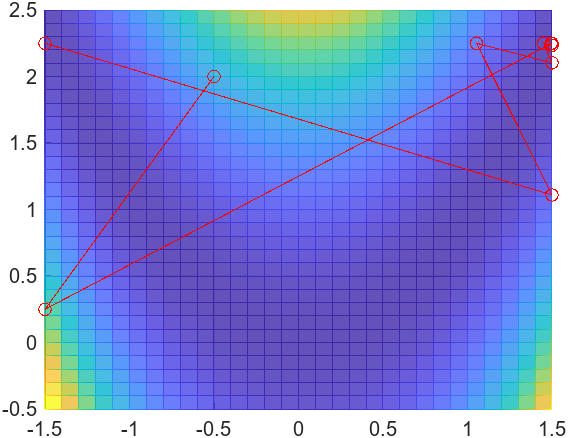
\includegraphics[width=0.4\textwidth]{divergence}
	\caption{Gradiens módszer divergenciája túl nagy tanulási ráta esetén}
\end{figure}
A módszer felparaméterezését és alkalmazhatóságát a szimulációs eredményeknél tárgyalom.

\subsection{Adam sztochasztikus gradiens módszer}
Az Adam \cite{Adam} egy sztochasztikus gradiens módszer. Minden lépésben adaptívan változtatja a tanulás paramétereit. Ezekek közül $m_t$ egy tapasztalati momentum, melyet a korábbi gradiensek exponenciálisan csökkenő súlyozásával kapunk. Hasonlóan számítandó $v_t$, mely a gradiensek négyzetének súlyozott átlaga, avagy a tapasztalati szórás. Legyen $g_t$ a gradiens, ekkor
$$ m_t = \beta_1 m_{t-1} + (1-\beta_1)g_t $$
$$ v_t = \beta_2 v_{t-1} + (1-\beta_2)g^2_t $$
Ahol $\beta_1$ és $\beta_2$ a módszer hiperparaméterei. A paraméterek a gyakorlatban a kezdeti értékük felé (általában 0) statisztikai ferdeséget (bias) mutatnak, ezért korrigálni kell őket:
$$ \hat{m_t} = \frac{m_t}{1-\beta_1^t} $$
$$ \hat{v_t} = \frac{v_t}{1-\beta_2^t} $$
Ezután egy lépés szabálya:
$$ a_{n+1} = a_n - \frac{\alpha}{\sqrt{\hat{v_t}}+\varepsilon}\hat{m_t} $$
A hiperparaméterekre a cikk szerzői ezeket az értékeket javasolják: $\alpha=0.002$ $\beta_1=0.9$ $\beta_2=0.999$ és $\varepsilon=10^{-6}$. Ezeket szimulációs eredmények alapján állítottam be az saját alkalmazáshoz. Mivel a GPU-n a dupla pontosságú lebegőpontos értékek számításigényesebbek, így shader környezetben nagyobb $\varepsilon$-t kell használni a numerikus stabilitás érdekében.

\subsection{AdaMax variáns}
Ezt a módosítást a cikk \cite{Adam} szerzői a cikk végén írják le. A lényege, hogy a szórás számításánál a kettes norma kicserélhető végtelen normára. Ezután a frissítés szabálya átalakítható max függvénnyé: (Itt $v_t$-t $u_t$-re cseréljük a megkülönböztethetőség kedvéért)
\begin{align*} 
	u_t &= \beta_2 u_{t-1} + (1-\beta_2)\norm{g_t}_\infty \\ 
	u_t &= \max (\beta_2 u_{t-1}, |g_t|)
\end{align*}
Az AdaMax frissítési szabálya ennek felhasználásával:
$$ a_{n+1} = a_n - \frac{\alpha}{u_t}\hat{m_t} $$
Végül ezt a variánst implementáltam GPU-n, mivel a számítása egyszerűbb és numerikusan stabilab, illetve mert néhány iterációval jobb eredményt ért el a szimuláció során. 


\section{Vetített gradiens módszer}

Előfordul, hogy az optimalizációs problémát a paramétertér csak egy kis részén kívánjuk megoldani. Például Bézier-felületeknél általában a $[0,1]$ intervallumon. Ebben az esetben nem elég az optimalizáció végén levetíteni az eredményt, ugyanis az a legtöbb esetben nem egyezik meg a tartományon vett minimumhellyel. \cite{MirrorDescent} Az sem jó, ha a lépés megtétele után vetítjük le a pontot a tartományra, ekkor ugyanis a gradiens módszer helytelen adatokkal fog számolni. 

Már a gradiens számításakor figyelembe kell venni a korlátokat. Legyen $g$ a gradiens, $\pi_C()$ pedig egy függvény, ami minden pontot a hozzá legközelebbi $C$ tartománybeli pontba visz. A vetített gradiens így számítható:
$$ g_p = (a_n - \pi_C(a_n-\varepsilon g))/\varepsilon $$
Ahol $\varepsilon$ egy kis szám. Ez úgy értelmezhető, hogy a gradiens irányába megteszünk egy kis lépést, majd azt levetítjük a tartományra. A vetített pont és az előző pont különbségéből megkapjuk a vetített gradienst irányát.

Ezt odaadjuk a gradiens módszerünknek, majd a lépés után ismét levetítjük. 

\cleardoublepage

% ------------------------------------------------------
\chapter{Fejlesztői dokumentáció}
\label{ch:developer}
% ------------------------------------------------------

% ------------------------------------------------------
% \chapter{Elméleti háttér}
% ------------------------------------------------------

\section{Elméleti háttér}

A következő fejezetekben a dolgozat elméleti hátterét ismertetem. 

\section{Sphere tracing}

A sugárkövetéssel történő képszintézisről részletes összefoglaló olvasható Bálint Csaba OTDK dolgozatában \cite[11-16. o.]{BalintCsaba}, így azt itt nem részletezem.

Adott egy $d:\mathbb{R}^n\rightarrow\mathbb{R}$ előjeles távolságfüggvény, mely minden bemenetre a pont a felület határától vett előjeles távolságát adja. Ez az érték a felület által határolt térrész belsejében negatív, kívül pedig pozitív. Formálisan $d$ akkor távolságfüggvény, ha az alábbi teljesül \cite{Hart1996}:
$$f(p) = d(p, f^{-1}(0)) (p \in \mathbb{R}^n)$$

A sugárkövetés során adott egy kiinduló pont és egy sugárirány. A cél a félegyenes és a felület metszéspontjának megtalálása. Míg a sugármetszés egyszerűbb matematikai objektumok esetén (pl. gömb, sík) analitikusan elvégezhető, bonyolultabb testek esetén csak óvatosabban közelíthetünk a felülethez a sugáron. (Ray Marching\cite{RayMarching})

A sphere trace algoritmusról Hart cikkében \cite{Hart1996} részletesen olvashatunk. Röviden összefoglalva a sphere trace egy sugárkövető algoritmus, mely minden lépésben kiértékeli a távolságfüggvényt. Tudjuk, hogy a távolságfüggvénnyel megegyező méretű üres tér van a pont körül, hiszen az a felülethez vett távolság minimumát vagy annak \emph{alsó közelítését} adja. Ekkor a távolsággal megegyező méretűt léphetünk a sugár mentén. A sugárkövetés a felület közelében lelassul. Ha a távolság epszilonnál kisebb lesz, vagy elértünk egy fix lépésszámot, akkor leállítjuk az iterációt.  


\section{Előjeles távolságfüggvények}


\subsection{Egyszerűbb alakzatok}
Inigo Quilez oldalán \cite{QuilezDistanceFunctions} felsorolja sok egyszerűbb alakzat analitikus távolságfüggvényét. Például egy $o$ középpontú és $r$ sugarú gömb előjeles távolságfüggvénye:
$$ d_{g}(p) = \norm{p-o}_2 - r $$
A weboldalon további testek távolságfüggvényei is láthatók. Ezekből aztán könnyen építhetünk színteret az alábbi tömörtest-modellezésben is használt műveletekkel: (Legyen az $A$ testtől vett előjeles távolságfüggvény $d_A$, a $B$ testtől vett pedig $d_B$)

\begin{itemize}
	\item Mivel a távolságfüggvény a legközelebbi távolságot adja, két test uniója a távolságfüggvények minimuma. $d(A\cup B) = min(d_A, d_B)$
	\item  Egy test ,,kifordítható'', ha a távolságfüggvény $-1$-szeresét vesszük $d\left(\overline{A}\right) = -d_A$.
	\item Két test metszete a távolságfüggvények maximuma, hiszen addig haladhatunk a sugár mentén, amíg mindkét alakzatot el nem találjuk. $d(A\cap B) = max(d_A, d_B)$
	\item Kivonást is végezhetünk, ha a test és a kifordított test metszetét vesszük. $d(A\backslash B) = max(d_A,-d_B)$ 
\end{itemize}

Elvégezhetők még a testeken transzformációk, ami általában a mintavételezési pontra alkalmazott inverz-transzformációval történik. Ilyenek például a nagyítás, nyújtás, lekerekítés, forgatás, kétdimenziós alakzat kiterjesztése hasábbá vagy forgástestté.

Különösen érdekes a tükrözés, ami az abszolútérték-függvénnyel elvégezhető, illetve az alakzat véges és végtelen ismétlése, melyet a koordinátákra alkalmazott moduló operátorral lehet elérni. \cite{QuilezDistanceFunctions}


\subsection{Parametrikus felületek távolságfüggvénye}

Háromdimenziós euklideszi térben parametrikus egyenlettel megadott felületeket hívjuk így. $f:\mathbb{R}^2\rightarrow\mathbb{R}^3$ Azért felület, mert a vektorértékű függvény értelmezési tartománybeli pontjaihoz háromdimenziós pontokat rendelünk. Modellezéskor így a test felszínét adjuk meg.  Például a tórusz parametrikus egyenlete:
$$ f(u,v) = \begin{pmatrix} 
	r\cdot sin(v) \\ 
	(R+r\cdot cos(v))\cdot sin(u) \\ 
	(R+r\cdot cos(v))\cdot cos(u)
\end{pmatrix} $$
Ahol $r$ a generáló kör sugara, $R$ pedig a forgástengely és a kör középpontjának távolsága. $u$ és $v$ szögek, így $u,v\in[0,2\pi]$.  
Parametrikus egyenlettel megadhatók függvények grafikonjai is. Legyen $h(u,v)$ a függvény, ekkor a grafikon parametrikus egyenlete:
$$ f(u,v) = (u,v,h(u,v)) $$
\begin{figure}[H]
	\centering
	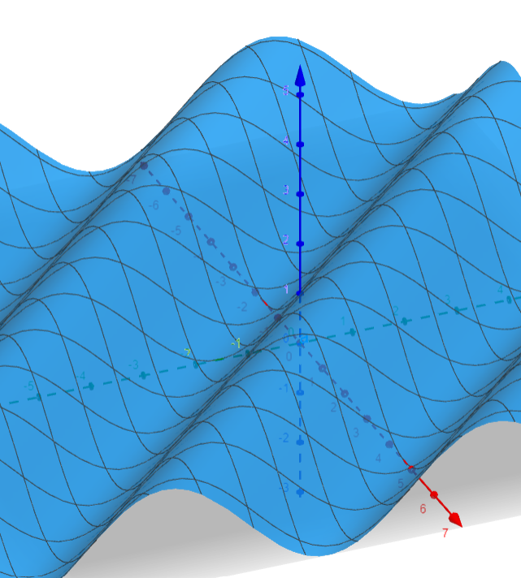
\includegraphics[width=0.3\textwidth]{sinuv}
	\caption{$h(u,v) = sin(u+v)+1$ grafikon a GeoGebra alkalmazásban.}
\end{figure}

Ezen felületek távolságfüggvénye analitikusan sok esetben nem meghatározható. Vegyünk egy kétdimenziós példát, az $y = sin(x)$ függvényt és egy $(e,f)$ mintavételezési pontot, amihez a legközelebbi pontot keressük a felületen. Ekkor a minimalizálandó függvény: 
$$ d(x) = \sqrt{(x-e)^2+(sin(x)-f)^2} $$
A gyök függvény szigorú monotonitása miatt vizsgáljuk $d^2$ minimumát. Az elsőrendű szükséges feltétel: 
$$ cos(x)\cdot(sin(x)-f)+x-e = 0 $$ 
Ezt csak néhány speciális esetben tudjuk analitikusan megoldani.

Polinomokkal sem boldogulunk könnyen analitikus módszerekkel. Például, ha a polinom fokszáma harmadfokú, akkor a négyzetre emelés és deriválás után egy ötödfokú polinom gyökeit kellene meghatározni. Erre már nem létezik megoldóképlet. Ez az eset előkerül a dolgozatomban a Bézier-felületek tárgyalásánál.


\section{Bézier-görbék}

Ennek a résznek alapul G. Farin: Curves and Surfaces for CAGD című könyve szolgált. \cite{farin2002curves} A de Casteljau-algoritmusról és Bézier-görbékről a könyv 45-47., a Bernstein-polinomokról a könyv 57. oldalán olvashatunk. Ezeket itt nem részletezem, csak a szükséges tételeket mutatom be. 

\subsection{Bernstein-alak}
Az $i$-edik $n$-edfokú Bernstein-polinom alakja:
$$ B^n_i(t) = \binom{n}{i}t^i(1-t)^{n-i} $$
Legyenek egy $n$-edfokú Bézier-görbe kontrollpontjai $b_0,b_2,\dots,b_n$ Ekkor a görbe felírható Bernstein-bázisban:
$$ b(t) = \sum_{i=0}^n b_i B^n_i(t) $$
Ezt a görbe Bernstein-alakjának is nevezik

\subsection{Végpont-interpoláció}
A Bernstein-polinomok tulajdonságaiból adódik, hogy a görbe a végpontjaiban egyenlő a szélső kontrollpontokkal, azaz interpolál.

\subsection{Pszeudolokális kontroll}
A legfontosabb tulajdonsága ezen görbéknek, hogy egy kontrollpont megváltoztatása csak annak környezetét változtatja meg jelentősen. Ennek oka, hogy $B^n_i(t)$-nek egyetlen maximuma van, a $t = i/n$ helyen. \cite[62. o.]{farin2002curves}

A végpont-interpoláció és a pszeudolokális kontroll miatt a görbe különösen alkalmas számítógépes modellezésre, mivel a felület a kontrollponthálójával intuitívan manipulálható.

\subsection{Derivált}
A görbe deriváltja: \cite[63. o.]{farin2002curves}
$$ b'(t) = n\sum_{i=0}^{n-1} \Delta b_i B^{n-1}_i(t) $$
Ahol $\Delta b_i = b_{i+1} - b_i$ ($\Delta$ a jobboldali differenciaoperátor.)



\section{Bézier-felületek}

\subsection{Bilineáris interpoláció}
Farin a Bézier-felületeket a tenzorszorzat-felületek bevezetéseként írja le. Egy egyik irámyban $m$, másik irányban $n$-edfokú felületet $(m+1)\cross(n+1)$ kontrollpont definiál. A felület pontjai kiszámíthatók a kontrollpontháló ismételt bilineáris interpolációjával. Ezt a felület pontbeli kiértékelésének nevezzük.

\begin{figure}[H]
	\centering
	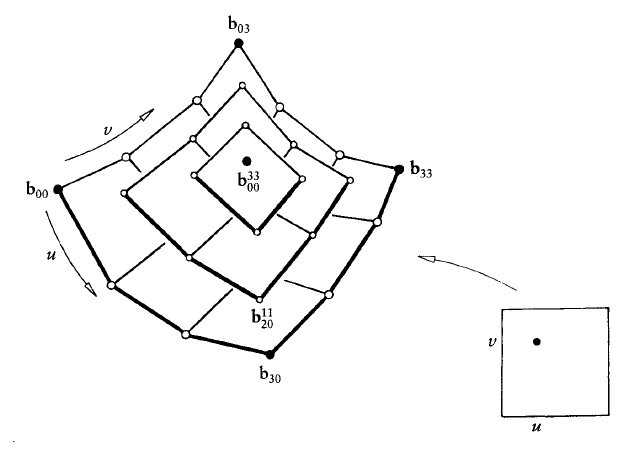
\includegraphics[width=0.5\textwidth]{Farin_bilinear}
	\caption{Bézier-felület kiértékelése \cite[248. o.]{farin2002curves}}
\end{figure}

\subsection{Bernstein-alak}
A végeredmény szempontjából lényegtelen, hogy az interpolációkat milyen sorrendben végezzük. Például kiértékelhetjük a kontrollponthálót az egyik paraméter szerint, majd az így keletkezett kontrollpontok által definiált Bézier-görbét a másik paraméter szerint. \cite[251. o.]{farin2002curves} A felület Bernstein-alakja:
$$ b^{m,n}(u,v) = \sum_{i=0}^m \sum_{j=0}^n b_{i,j}\, B^m_i(u) B^n_j(v) $$

\subsection{Parciális deriváltak}
A könnyebb leírás érdekében bevezetjük a parciális differenciaoperátort. Ennek szabályai: $\Delta^{1,0}b_{i,j} = b_{i+1,j} - b_{i,j}$ és  $\Delta^{0,1}b_{i,j} = b_{i,j+1} - b_{i,j}$

A parciális deriváltat a Bézier-görbe deriváltjára vezetjük vissza:
$$ \partial_u b^{m,n}(u,v) = \sum_{j=0}^n \left[\partial_u \sum_{i=0}^m b_{i,j} B^m_i(u) \right] B^n_j(v) $$
$$ \partial_u b^{m,n}(u,v) = m\sum_{j=0}^n \sum_{i=0}^{m-1} \Delta^{1,0} b_{i,j} B^{m-1}_i(u)  B^n_j(v) $$
A másik parciális derivált hasonlóan meghatározható:
$$ \partial_v b^{m,n}(u,v) = n\sum_{j=0}^{n-1} \sum_{i=0}^m \Delta^{0,1} b_{i,j} B^m_i(u)  B^{n-1}_j(v) $$
Magasabbrendű deriváltakat a dolgozatban nem használtam, így azokat itt nem tárgyalom. Az általános alak szintén megtalálható Farin könyvében. \cite[257. o.]{farin2002curves}



\section{Legközelebbi pont meghatározása}

A legközelebbi pont meghatározása nem egyszerű feladat. Egyszerűsítésként egy $b(x,y)$ függvény grafikonjára próbáljuk meg meghatározni. Ezen belül is vegyünk egy harmadfokú Bézier-felületet.

\subsection{Merőlegesség feltétel}
A legközelebbi pont szükséges feltétele: Az $E$ mintavételezési pontból a felületi pontba húzott egyenes merőleges mindkét parciális deriváltra. Egyik irányra felírva:
$$ r(x,y) = (x,y,b(x,y)) $$
$$ \frac{dr}{dx} = (1,0,b_x(x,y)) $$
Ahol $b_x$ az első koordináta szerinti parciális derivált. A mintavételezési pont legyen az origó. Ezt megtehetjük, hiszen a felületet átparaméterezhető úgy, hogy a mintavételezési pont az origóba essen. Ha két vektor merőleges, a skalárszorzatuk $0$.
$$ 0 = \left\langle r, \frac{dr}{dx} \right\rangle = \begin{pmatrix} 1 $ 0 $ b_x(x,y) \end{pmatrix} \cdot \begin{pmatrix} x \\ y \\ b(x,y)\end{pmatrix} = x + b_x(x,y)b(x,y) $$
$x$ szerint parciálisan integrálva: 
$$ f(y) = x^2/2 + b(x,y)^2 $$
$$ x=0 \rightarrow f(y) = b(0,y)^2 $$
$$ b(0,y)^2 = x^2/2 + b(x,y)^2 $$
A feltétel barátságos alakja ellenére a mi esetünkben (harmadfokú Bézier) ez egy ötödfokú kétismeretlenes egyenlet tetszőleges együtthatókkal. 

Látjuk, hogy ez a megközelítés nem vezet eredményre. Ugyanezt az egyenletet kapjuk, ha a szükséges feltételt a felületi normális segítségével írjuk fel. Ezt itt nem részletezem. Az algoritmusok résznél a problémára több közelítési módszert is bemutatok.

% ------------------------------------------------------
% \chapter{Algoritmusok}
% ------------------------------------------------------

\section{Fénymodell}

Fénymodellnek egy egyszerű Blinn-Phong árnyalást használtam \cite{Blinn1977} árnyéksugarakkal. Az árnyéksugár számítás ugyanazt az algoritmust használja, mint a sugárkövetés. Ha elmetsszük a felületet a felületi pontból a (pont)fényforrás felé indított sugárral, akkor a felületi pont árnyékban van.

Fontos megemlíteni, hogy a távolságfüggvények segítségével puha árnyékszámító algoritmus is adható. \cite{AreaLights}


\section{Távolságfüggvény rács számítása}

A távolságfüggvényt egy diszkrét rácson értékelem ki, melyet egy háromdimenziós textúrában tárolok. Mivel csak a mintavételezési pont változik, maga a kiértékelendő (vagy meghatározandó) távolságfüggvény nem, így ki tudom használni a GPU masszívan párhuzamos architektúráját. A textúrát saját GPU compute shaderek segítségével számítom ki. A számítás elvégzésére később több módszert is mutatok. 

Fontos megjegyezni, hogy ennek a műveletnek nem kell valós idejűnek lennie. A program indításakor a textúra több frame alatt kiszámítható. Ezután elég a textúrát a fragment shader számára feltölteni a GPU-ra a sugárkövetés előtt.


\section{Sugárkövetés távolságmezőn}

A sugárkövetés során adott a kiinduló pont $P$, és a sugár iránya $d$. Emellett adott egy $F$ függvény, mely az előbb részletezett textúra olvasást és bilineáris interpolációt elvégzi, majd visszaadja a távolságfüggvény becslését. A távolságfüggvény rácsból az értékeket a textúra bilineáris interpolációjával nyerem ki. Ez a fajta textúra mintavételezés egy hardveresen támogatott művelet a GPU-n. Az alábbi függvény a kiindulási pont és a sugár felülettel vett első metszéspontjának távolságát adja meg.

\begin{algorithm}[H]
	\caption{Sugárkövetés távolságmezőn}
	\label{alg:ibb}
	\textbf{\underline{Funct}} SDFBoxTrace($P,d,F$)
	\begin{algorithmic}[1] % sorszámok megjelenítése minden n. sor előtt, most n = 1
		\If{$P$ a dobozon kívül van}
		\State{\textbf{return} $-1$} \Comment{Távolság nem definiált}
		\EndIf
		\If{$F(P) \leq 0$}
		\State{\textbf{return} $0$} \Comment{A doboz oldalán már a felületben vagyunk}
		\EndIf
		\State{$depth := 0$}
		\For{$i \gets 1$ to maxSteps} \Comment{Maximum lépésszám}                    
		\State{$dist := F(P + depth * d)$}
		\If{$abs(dist) < \varepsilon$}
		\State{\textbf{return} $depth$} \Comment{Eltaláltuk a felületet}
		\EndIf
		\State{$depth\; +\! = dist$}
		\State{$currPos := P + depth * d$}
		\If{$currPos$ a dobozon kívül van}
		\State \textbf{return} $-1$; \Comment{Távolság nem definiált, nincs metszés}
		\EndIf
		\EndFor
		\State \textbf{return} $-1$; \Comment{Távolság nem definiált, nincs metszés}
	\end{algorithmic}
\end{algorithm}


\section{Egyszerűbb távolságfüggvény-számító algoritmusok}

Ebben a részben két egyszerűbb megközelítést mutatok be, melyek általánosan használhatók előjeles távolságfüggvények generálására.

\subsection{Lipschitz-módszer}
A módszer elméleti hátterét Bálint Csaba dolgozatából \cite[18. o.]{BalintCsaba} idézem: ,,$\dots$ ha $f \in \mathbb{R}^n \rightarrow \mathbb{R}$ függvény Lipschitz folytonos, akkor
$$ \frac{|f|}{Lip(f)} $$
távolságfüggvény becslés. Általában az abszolút érték elhagyható, hogy előjeles távolságfüggvényt kapjunk. Ezzel egy módszert kaptunk arra, hogy egy implicit függvényhez hogyan gyártsunk távolságfüggvényt. Sokszor a $Lip(f)$-et csak felülről tudjuk becsülni, vagy nem éri meg kiszámolni. Ilyenkor természetesen $f$-et a $Lip(f)$ felső becslésével osztva egy rosszabb becslést kapunk, amivel sokszor lényegesen lassabb a számolás.''

A módszerrel egy grafikon például megjeleníthető az alábbi módon:
\begin{itemize}
	\item Egy előre meghatározott felbontású rácson kiértékeljük a függvényt. Ezzel egy magasságtérképet generálunk.
	\item Megbecsüljük a Lipschitz-konstanst a számolt értékekből vagy megadjuk analitikusan, ha ismert.
	\item A távolságmező minden eleme a pont magasságtérképtől vett távolsága lesz, $Lip(f)$-el leosztva. Ezzel távolságfüggvény-becslést kapunk.
\end{itemize}

\subsection{Brute force}
A felületet valamilyen felbontáson kiértékeljük. A legközelebbi pont távolságát eltároljuk a távolságmezőben. A módszer hátránya, hogy a számítási igény négyzetesen nő a felbontás növelésével. (Amellett, hogy a háromdimenziós rács minden pontjára külön ki kell számolni.)

A módszer előnye, hogy a távolságmező (a felbontás limitációja mellett) pontos és maximális lesz. A távolságmező minden pontjára igaz, hogy az értéke nem növelhető, hiszen minden pontra létezik olyan sugár, melyen az ott tárolt távolságot lépve a felület egy ismert pontjába lépünk. Ezen tulajdonság miatt a sugárkövetésnek sokkal kevesebb lépésre van szüksége a felület megtalálására. A bemutatott két módszer közül a brute force a preferált, hiszen a távolságmező előszámítható és akár el is tárolható háttértáron.


\section{Gradiens módszerek}

A felülettől vett minimális távolság valójában egy optimalizációs probléma. Optimalizációs problémák megoldásának nagyon széles szakirodalma van. Ilyen problémát kell megoldani többek között neuronhálók tanításánál is. 2020-ban távolságfüggvényekkel való ütközésdetektálás javítására is használtak lokális optimalizációt. \cite{locOptSDFCollision} A távolságfüggvényekhez két, a gépi tanulásban elterjedt algoritmust is implementáltam.

\subsection{Gradiens módszer}
A gradiens módszer egy elsőrendű iteratív optimalizációs algoritmus. A módszer alapötletét egészen Cauchy-ig vezetik vissza \cite{LemarechalOnGrad}, így egyáltalán nem újszerű. Az iteráció egy lépése:
$$ a_{n+1} = a_n - \alpha\nabla F(a_n) $$
Ahol $F$ a minimalizálandó függvény, $\nabla$ a gradiens-operátor és $\alpha$ a tanulási ráta. $\alpha$ egy kis konstans, ami a módszer konvergenciáját biztosítja. Ha túl nagyra állítjuk, akkor a módszer nem konvergál. 
\begin{figure}[H]
	\centering
	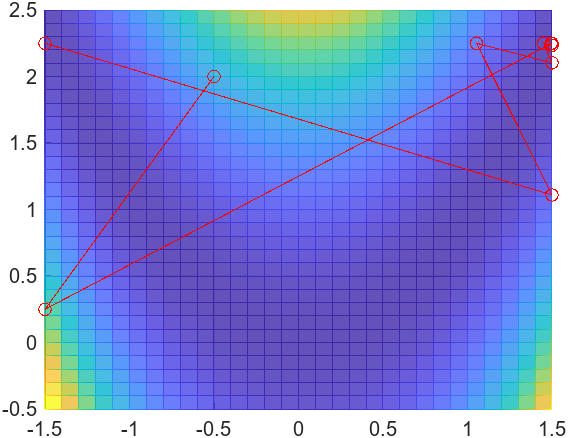
\includegraphics[width=0.4\textwidth]{divergence}
	\caption{Gradiens módszer divergenciája túl nagy tanulási ráta esetén}
\end{figure}
A módszer felparaméterezését és alkalmazhatóságát a szimulációs eredményeknél tárgyalom.

\subsection{Adam sztochasztikus gradiens módszer}
Az Adam \cite{Adam} egy sztochasztikus gradiens módszer. Minden lépésben adaptívan változtatja a tanulás paramétereit. Ezekek közül $m_t$ egy tapasztalati momentum, melyet a korábbi gradiensek exponenciálisan csökkenő súlyozásával kapunk. Hasonlóan számítandó $v_t$, mely a gradiensek négyzetének súlyozott átlaga, avagy a tapasztalati szórás. Legyen $g_t$ a gradiens, ekkor
$$ m_t = \beta_1 m_{t-1} + (1-\beta_1)g_t $$
$$ v_t = \beta_2 v_{t-1} + (1-\beta_2)g^2_t $$
Ahol $\beta_1$ és $\beta_2$ a módszer hiperparaméterei. A paraméterek a gyakorlatban a kezdeti értékük felé (általában 0) statisztikai ferdeséget (bias) mutatnak, ezért korrigálni kell őket:
$$ \hat{m_t} = \frac{m_t}{1-\beta_1^t} $$
$$ \hat{v_t} = \frac{v_t}{1-\beta_2^t} $$
Ezután egy lépés szabálya:
$$ a_{n+1} = a_n - \frac{\alpha}{\sqrt{\hat{v_t}}+\varepsilon}\hat{m_t} $$
A hiperparaméterekre a cikk szerzői ezeket az értékeket javasolják: $\alpha=0.002$ $\beta_1=0.9$ $\beta_2=0.999$ és $\varepsilon=10^{-6}$. Ezeket szimulációs eredmények alapján állítottam be az saját alkalmazáshoz. Mivel a GPU-n a dupla pontosságú lebegőpontos értékek számításigényesebbek, így shader környezetben nagyobb $\varepsilon$-t kell használni a numerikus stabilitás érdekében.

\subsection{AdaMax variáns}
Ezt a módosítást a cikk \cite{Adam} szerzői a cikk végén írják le. A lényege, hogy a szórás számításánál a kettes norma kicserélhető végtelen normára. Ezután a frissítés szabálya átalakítható max függvénnyé: (Itt $v_t$-t $u_t$-re cseréljük a megkülönböztethetőség kedvéért)
\begin{align*} 
	u_t &= \beta_2 u_{t-1} + (1-\beta_2)\norm{g_t}_\infty \\ 
	u_t &= \max (\beta_2 u_{t-1}, |g_t|)
\end{align*}
Az AdaMax frissítési szabálya ennek felhasználásával:
$$ a_{n+1} = a_n - \frac{\alpha}{u_t}\hat{m_t} $$
Végül ezt a variánst implementáltam GPU-n, mivel a számítása egyszerűbb és numerikusan stabilabb, illetve mert néhány iterációval jobb eredményt ért el a szimuláció során. 


\section{Vetített gradiens módszer}

Előfordul, hogy az optimalizációs problémát a paramétertér csak egy kis részén kívánjuk megoldani. Például Bézier-felületeknél általában a $[0,1]$ intervallumon. Ebben az esetben nem elég az optimalizáció végén levetíteni az eredményt, ugyanis az a legtöbb esetben nem egyezik meg a tartományon vett minimumhellyel. \cite{MirrorDescent} Az sem jó, ha a lépés megtétele után vetítjük le a pontot a tartományra, ekkor ugyanis a gradiens módszer helytelen adatokkal fog számolni. 

Már a gradiens számításakor figyelembe kell venni a korlátokat. Legyen $g$ a gradiens, $\pi_C()$ pedig egy függvény, ami minden pontot a hozzá legközelebbi $C$ tartománybeli pontba visz. A vetített gradiens így számítható:
$$ g_p = (a_n - \pi_C(a_n-\varepsilon g))/\varepsilon $$
Ahol $\varepsilon$ egy kis szám. Ez úgy értelmezhető, hogy a gradiens irányába megteszünk egy kis lépést, majd azt levetítjük a tartományra. A vetített pont és az előző pont különbségéből megkapjuk a vetített gradienst irányát.

Ezt odaadjuk a gradiens módszerünknek, majd a lépés után ismét levetítjük. 



% ------------------------------------------------------
% \chapter{Szimulációs eredmények}
% ------------------------------------------------------

\section{Szimulációs eredmények}

GPU környezetben nehéz algoritmusokat tesztelni és hibákat javítani, a masszívan párhuzamos környezet miatt, ezért az algoritmusokat egy szálon, Matlabban is implementáltam. A vizsgálat középpontjában az algoritmusok stabilitása és konvergenciája állt. 

\section{Gradiens módszerek stabil paraméterezése}

A gradiens módszer egyszerűsége ellenére meglepően jól teljesít Bézier felületeken abban az esetben, ha a tanulási rárát ($\alpha$) a lehető legnagyobb értékre állítjuk. Ekkor azonban nem tudunk garantálni semmiféle konvergenciát. Emiatt olyan hiperparaméter-beállítást keresünk, mely szélsőséges esetben is a lokális minimumhoz konvergál.

\subsection{Rosenbrock-függvény}
A Rosenbrock-függvény egy klasszikus "nehéz" példa, melyet optimalizációs algoritmusok tesztelésére szoktak alkalmazni. Definíciója:
$$ f(x,y) = (a-x)^2 + b(y-x^2)^2 $$
Ennek a globális minimuma az $(a,a^2)$ helyen van. Az $a$ paraméter értéke általában $1$. A $b$ paraméterrel a probléma ,,nehézségét'' lehet állítani. Minél nagyobb a $b$ érték, annál nagyobb lesz a gradiensvektor hossza. Én $20$-ra állítottam.
\begin{figure}[H]
	\centering
	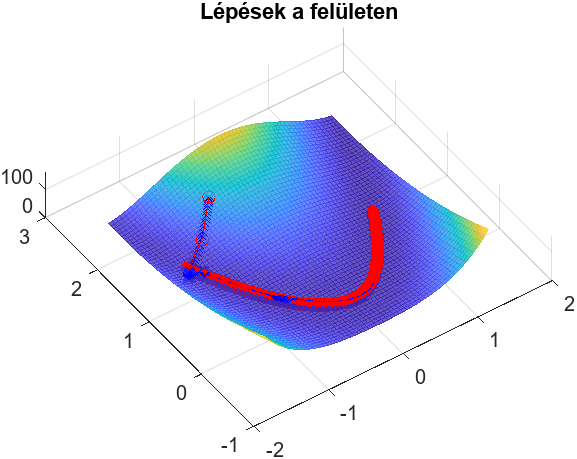
\includegraphics[width=0.4\textwidth]{RB_surf}
	\hspace{5pt}
	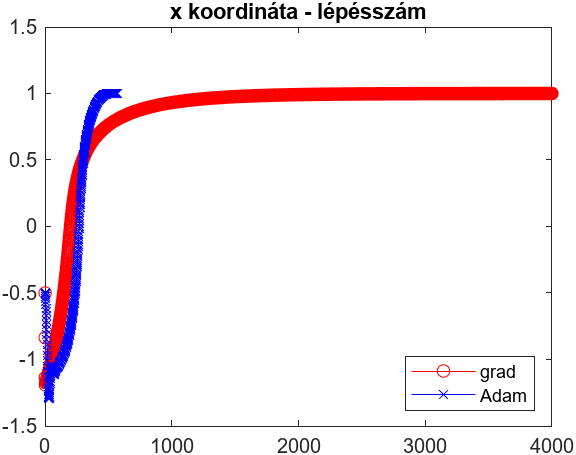
\includegraphics[width=0.4\textwidth]{RB_x}
	\caption{Stabil paraméterezés a Rosenbrock-függvényen}
	\label{fig:RB}
\end{figure}
A gradiens módszer paramétere: $\alpha = 0,005$ \\
Az AdaMax módszer paraméterei: $\alpha = 0,005$, $\beta_1 = 0,9$, $\beta_2 = 0,99$ \\
\Aref{fig:RB} ábrán pirossal a gradiens módszer lépéseit, kékkel az AdaMax módszer lépéseit jelöltem. Az AdaMax módszer $569$ lépésben $10^{-6}$ nagyságrendű hibával konvergál. A gradiens módszer hibája $1000$ lépés után $1/10$-nél nagyobb, és még $5000$ lépés után is $10^{-4}$ nagyságrendű.

Ebből a példából jól látszik a bonyolultabb módszer előnye, ha megköveteljük a konvergenciát nehezebb példákra is.



\section{Globális minimum harmadfokú Bézier-felületen}

A módszereket Bézier-felületeken is összehasonlítottam. A cél alapvetően a Bézier-felület távolságfüggvényének generálása. Ehhez a globális minimumot kell meghatározni. Ezt úgy kívánjuk elérni, hogy a lokális optimumkereső algoritmust több pontból elindítjuk. Az itt következő példák intuíciót adnak az indítási pontok minimális számára, amit a következő részben szimulációval validálok.

\subsection{Sarokpontok}
\Aref{fig:corners} példában az látszik, hogy lokális optimum közel lehet a felület sarkához ($(0,0),(0,1),(1,0),(1,1)$ pontok). Ha a felület belsejéhez tartozó kontrollpontok koordinátáit nagyobbra állítjuk, a baloldali ábrán látható lokális szélsőértékek tetszőlegesen közel kerülhetnek a sarokpontokhoz. 
\begin{figure}[H]
	\centering
	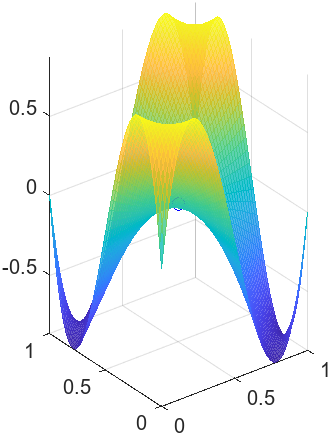
\includegraphics[height=0.35\textwidth]{sarokF.png}
	\hspace{5pt}
	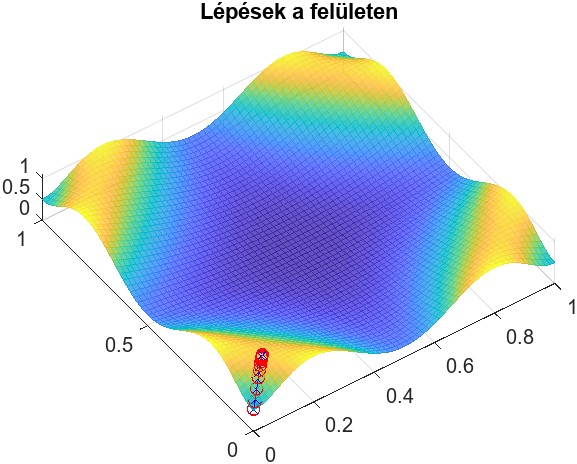
\includegraphics[height=0.35\textwidth]{sarokLep.png}
	\caption{Példa sarokpontok szükségességére}
	\label{fig:corners}
\end{figure}
A jobboldali ábrán a felület és az $(1/2,1/2,0)$ pont távolsága látható. Emellett a gradiens módszerek lépései szerepelnek az $(1/10,1/10)$ pontból indítva.

Ezen a példán az látszik, hogy a sarokpontokból el kell indítani a keresést, illetve hogy a felület belsejében lévő lokális minimumot nem lehet minden esetben a sarkokból megtalálni. Én ezért az $(1/2,1/2)$ pontot is hozzávettem a kiindulási pontokhoz.

\subsection{Oldalak}
Az alábbi példán az látszik, hogy a lokális minimum lehet az oldal mentén is, és azt nem feltétlenül találjuk meg a sarokpontból indulva.
\begin{figure}[H]
	\centering
	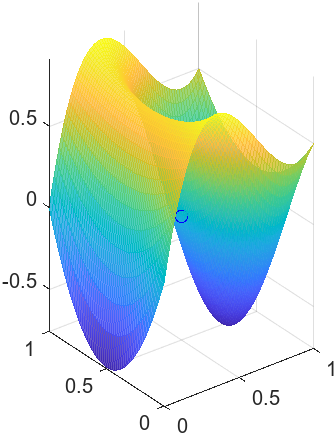
\includegraphics[height=0.3\textwidth]{oldalF.png}
\end{figure}
\begin{figure}[H]
	\centering
	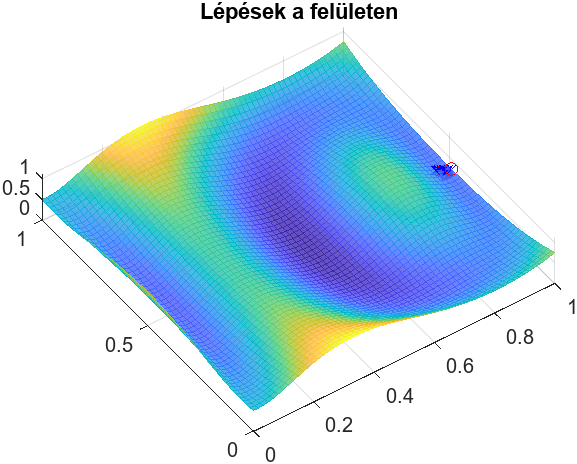
\includegraphics[height=0.35\textwidth]{oldalLep1.png}
	\hspace{5pt}
	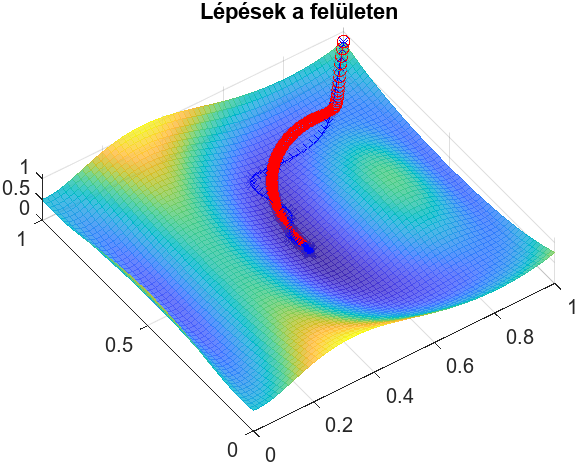
\includegraphics[height=0.35\textwidth]{oldalLep2.png}
	\caption{Példa oldalpontok szükségességére}
\end{figure}
Emiatt én az oldalak középpontját is hozzávettem a kiindulási pontokhoz.

\subsection{A 10 pont módszer}
$9$ indítási pont egy egyenletes $3\cross3$-as felosztás a paramétertérben. Ezzel a felület nagyobb vonásait lefedjük. Azért, hogy a módszer a felület közelében is gyorsan konvergáljon, a mintavételezési pont alatti felületi pontból is elindítom a keresést. Mivel grafikonon vagyunk, ez megegyezik az első két koordinátával.



\section{AdaMax algoritmus Bézier-felületeken}
A 10 pont módszer helyességét szimulációval kívánom igazolni. Ehhez nagyszámú mintát generáltam, majd ellenőriztem, hogy a javasolt módszer minden alkalommal megtalálta-e a globális minimumot.

\subsection{Felületgenerálás}
A harmadfokú Bézier-felületek generálásához elég a $4\cross4$ kontrollpontot megadni. Ehhez egyenletes eloszlással véletlen pontokat vettem a $[-1,1]$ intervallumból. Az így keletkező felületek a közepükön meglehetősen laposak voltak. Ennek oka, hogy amíg a  $0.$ és a $3.$ harmadfokú Bernstein-polinom maximuma az $1$ értéket veszi fel, addig a középsők maximuma csak $4/9$. Ez különösen látványos a felület közepén, ott ugyanis két Bernstein-polinom szorzata áll melyek maximuma $(4/9)^2$. Ezen tulajdonság miatt a középső kontrollpontoknak sokkal kisebb hatása van, mint a szélsőknek, ahol ráadásul interpolál is a felület. Emiatt minden kontrollpont harmadik koordinátáját leosztottam a hozzá tartozó Bernstein-polinom maximumával.

\subsection{Mintavételezési pont generálás}
A mintavételezési pontokat a felület bennfoglaló dobozából és annak környezetéből vettem. Ehhez egy egyenletes felosztású térrács pontjait random vektorokkal eltoltam. Az ábrán egy példa merőleges vetülete látható.
\begin{figure}[H]
	\centering
	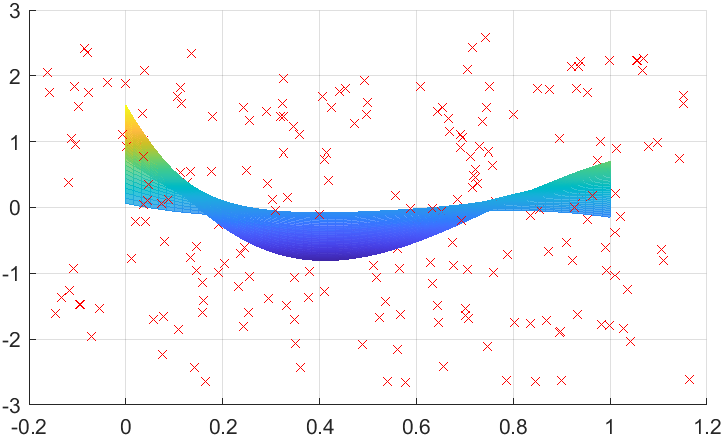
\includegraphics[width=0.5\textwidth]{mintavetel.png}
	\caption{Felület és ponthalmaz képe}
\end{figure}

\subsection{Referenciaértékek}
Referenciaértékként kiszámítottam minden mintavételezési pontra a ,,brute force'' módszer eredményét, azaz a távolságot egy $n\cross n$-es rácson kiértékeltem.
\begin{figure}[H]
	\centering
	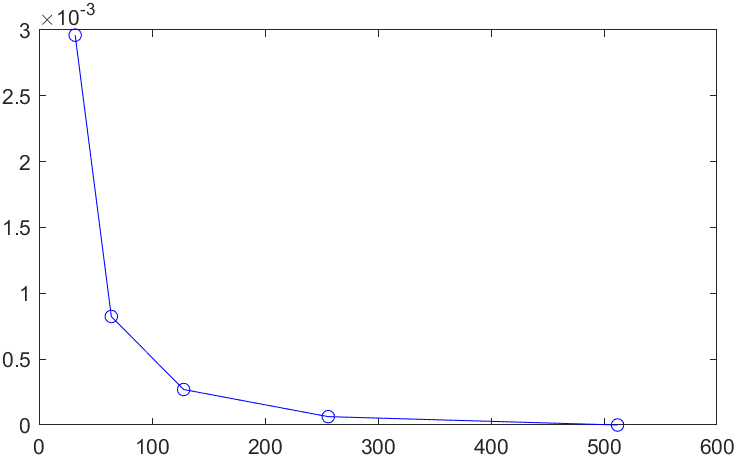
\includegraphics[width=0.5\textwidth]{ground_truth.png}
	\caption{Referenciaérték maximális hibája a legnagyobb felbontáshoz képest}
\end{figure}
A tesztek alapján a hiba a műveletigénnyel arányosan csökken, pontosabban a felbontás ($n$) duplázásakor a hiba közel a negyedére csökken. A továbbiakban az $n=256$ értéket használom.



\section{Validáció}

A $10$ pont algoritmust $1000$ különböző példára futtattam, majd összehasonlítottam a kapott minimumot a referenciaértékkel. Mivel azt szeretnénk, hogy az algoritmus a legrosszabb esetben is megadja az optimumot, azért a grafikonon az összes futtatás közül a relatív hiba maximumát ábrázoltam minden egyes lépésszámra.
\begin{figure}[H]
	\centering
	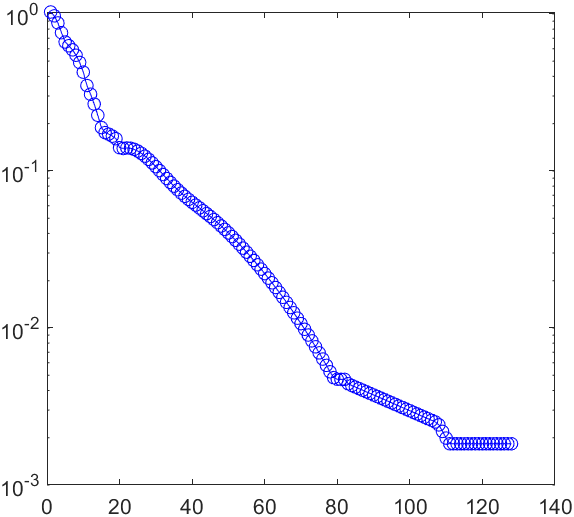
\includegraphics[width=0.5\textwidth]{stepcount.png}
	\caption{Abszolút hiba maximuma a lépésszám függvényében, logaritmikus skálán}
\end{figure}
A módszer minden futtatás esetén megtalálta az optimumot legalább a referenciaérték pontosságával, kevesebb, mint $120$ iteráció alatt. A grafikon $110$ lépés után azért laposodik el, mert az algoritmus eléri a referenciaérték pontosságát. Ha referenciának az utolsó iteráció által adott távolságot vesszük, akkor látható, hogy a módszer tovább konvergál.
\begin{figure}[H]
	\centering
	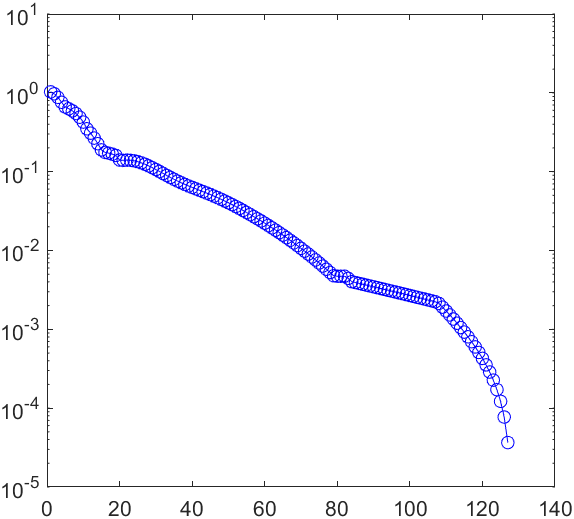
\includegraphics[width=0.5\textwidth]{005_8_99.png}
	\caption{Abszolút hiba maximuma az iteratív módszerhez viszonyítva.}
\end{figure}


\section{A program szerkezete}
A program szerkezete \aref{fig:szerkezet} ábrán látható. A program a Falcor keretrendszerre épít. A fő programot az SDFBox osztály tartalmazza, mely az adatok tárolására és manipulálására különböző osztályokat használ. Ezek felelőssége, az adatok tárolása mellett több esetben GPU-val való kommunikáció, mely magába foglalja az adatok feltöltését és a futtatás parancsok kiadását.

Az osztályokra mutató referenciákat * karakterrel jelöltem. A típusok között megjelennek float3, float4, float4x4, stb., melyek különböző méretű lebegőpontos számokat tartalmazó vektorokat és mátrixokat jelölnek.

\begin{figure}
	\centering
	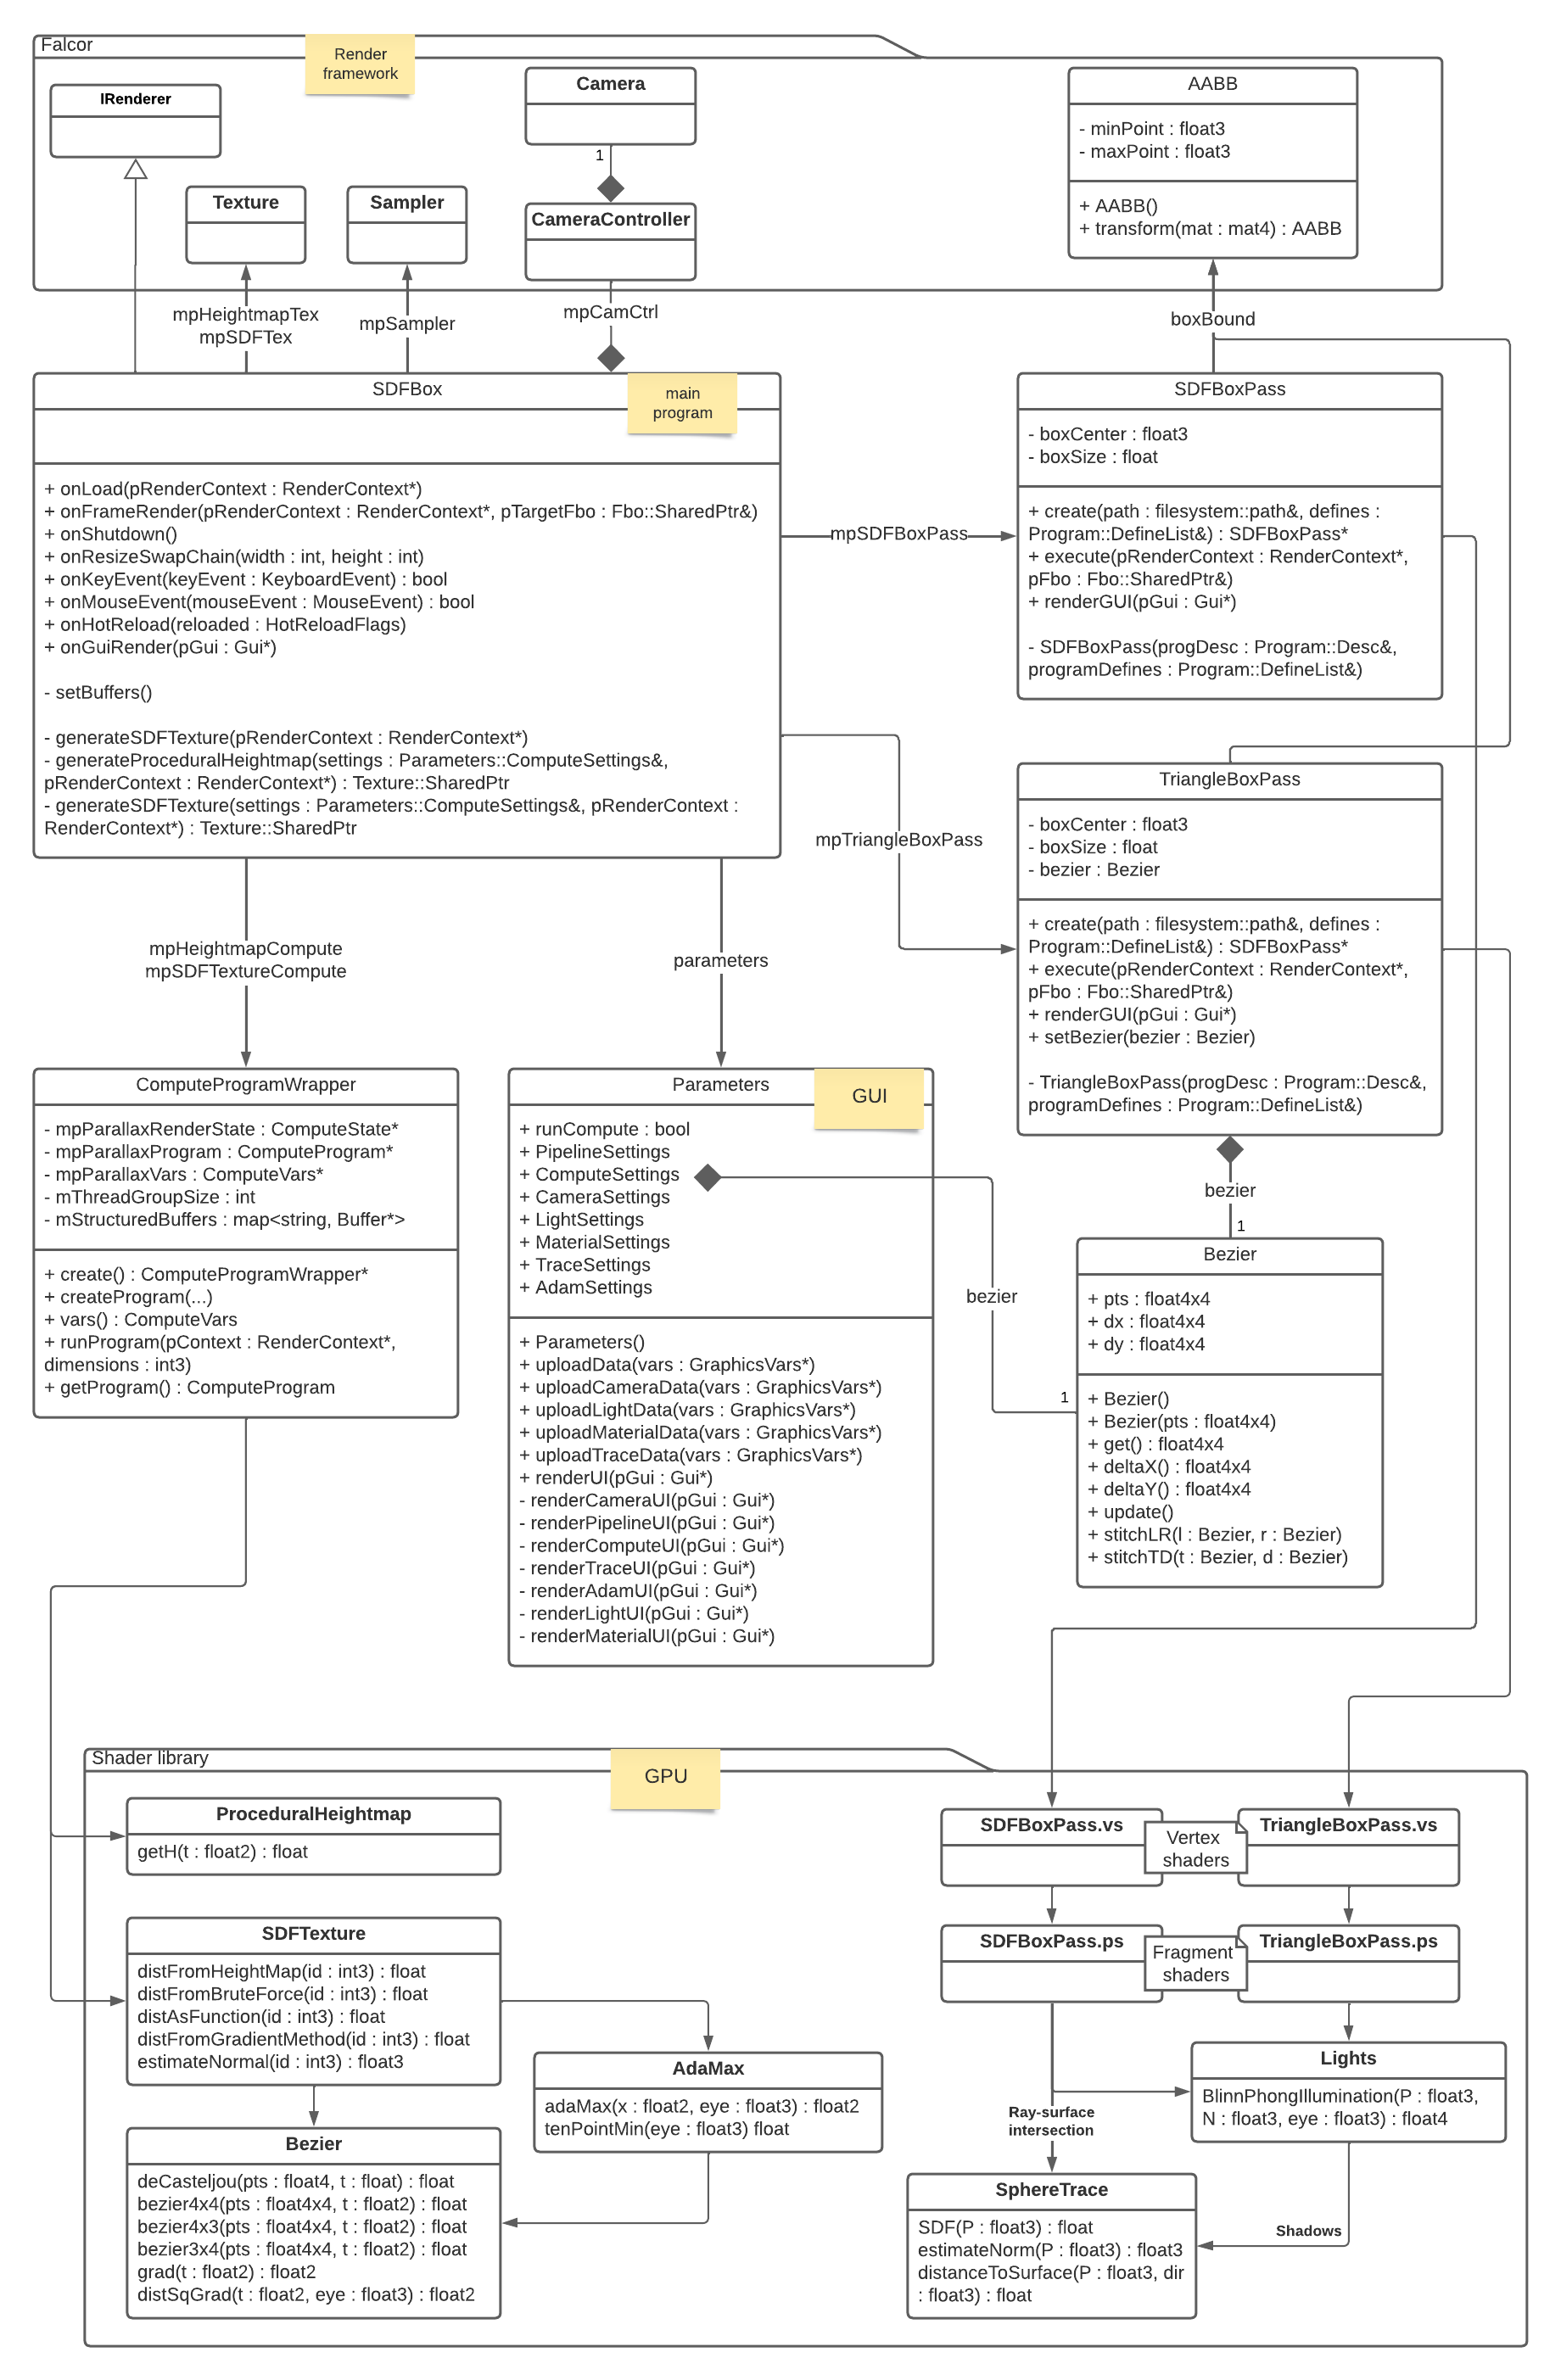
\includegraphics[width=1.0\textwidth]{szerkezet.png}
	\caption{A program szerkezete}
	\label{fig:szerkezet}
\end{figure}


\section{Osztályok}

\subsection{SDFBox}
A fő program, mely a Falcor keretrendszer IRenderer osztályából származik le. Annak fő metódusait írja felül, melyek a megfelelő szakaszban képkockánként vagy az adott esemény előfordulásakor meghívásra kerülnek. A függvények szerepe:
\begin{itemize}
	\item onLoad: A program indulásakor fut le. Itt lehet a saját adattagokat inicializálni.
	\item onFrameRender: Minden képkocka kirajzolása előtt lefut. A program fő része itt található.
	\item onShutdown: A program leállásakor fut le.
	\item onResizeSwapChain: Az ablak átméretezésekor fut le. Lehetőséget ad a kirajzolt elemek átméretezésére.
	\item onKeyEvent: Billentyűlenyomások kezelhetőek le itt.
	\item onMouseEvent: Egérbemenetet lehet lekezelni vele.
	\item onGuiRender: A felhasználói felület kirajzolása ImGui segítségével.
\end{itemize}

\subsection{SDFBoxPass}
Egy távolságmezőt tartalmazó kocka. Ez az osztály felelős a távolságmező kirajzolásáért és a kirajzolást végző grafikus program létrehozásáért és futtatásáért.

\subsection{TriangleBoxPass}
Egy háromszögekkel közelített Bézier-felület raszterizációval történő megjelenítését végzi. A kemény árnyékokhoz ugyanúgy szükség van a távolságmezőre, mint az SDFBoxPass esetében.

\subsection{ComputeProgramWrapper}
Egy compute shader futtatásához szükséges adatokat tárolja. A compute shader létrehozásához és futtatásához biztosít interfészt.

\subsection{Parameters}
A jelenetben található objektumok (fények, felületek, kamera) adatait és a generáláshoz szükséges paramétereket tárolja. Az adatokat szükség esetén feltölti a GPU-ra. A beállítások a felhasználói felületen keresztül futási időben is manipulálhatók.

\subsection{Bezier}
Egy Bézier-felület kontrollponthálóját tárolja. Lekérdező műveleteket ad a parciális differenciákra. Lehetővé teszi véletlen Bézier-felület generálását. A GPU oldali Bezier shader megfelelője.


\section{Shaderek}

\subsection{ProceduralHeightmap és SDFTexture}
A ProceduralHeightmap shader egy magasságtérkép elkészítéséért felel. A bemeneti adatokból magasságtérképet készít, melyet egy kimeneti textúrába ír. Az SDFTexture ebből a magasságtérképből vagy pedig bemeneti adatokból távolságmezőt generál, melyet egy kimeneti textúrában tárol.

\subsection{AdaMax és Bezier}
Az AdaMax shader az AdaMax gradiens módszer GPU implementációját tartalmazza. A shader gradiensként egy Bézier-felületet értékel ki. A függvénykiértékelést a Bezier shader végzi.

\subsection{Lights és SphereTrace}
A jelenetben pontfényforrások helyezhetőek el, melyeket a felület Blinn-Phong árnyalásával jelenítek meg. Az árnyalás számításáért a Lights shader felel. Bemeneti adatok a felületi pont, a felületi normális és a kamera pozíció. Az ún. kemény árnyékok számításához a SphereTrace shadert használom, mely egy távolságmezőn képes a sugár felülettel vett metszéspontját meghatározni.


\section{Felhasználói eset diagram}

A felhasználó a billentyűzettel, egérgesztusokkal és a grafikus felhasználói felületen keresztül interaktálhat a programmal. Ha egy számítás elvégzéséhez szükséges adat megváltozik, akkor az adatokat a CPU és a GPU oldalon is frissíteni kell és a számításokat újra el kell végezni. A felhasználói esetek diagramja \aref{fig:usecase} ábrán látható.
\begin{figure}[H]
	\centering
	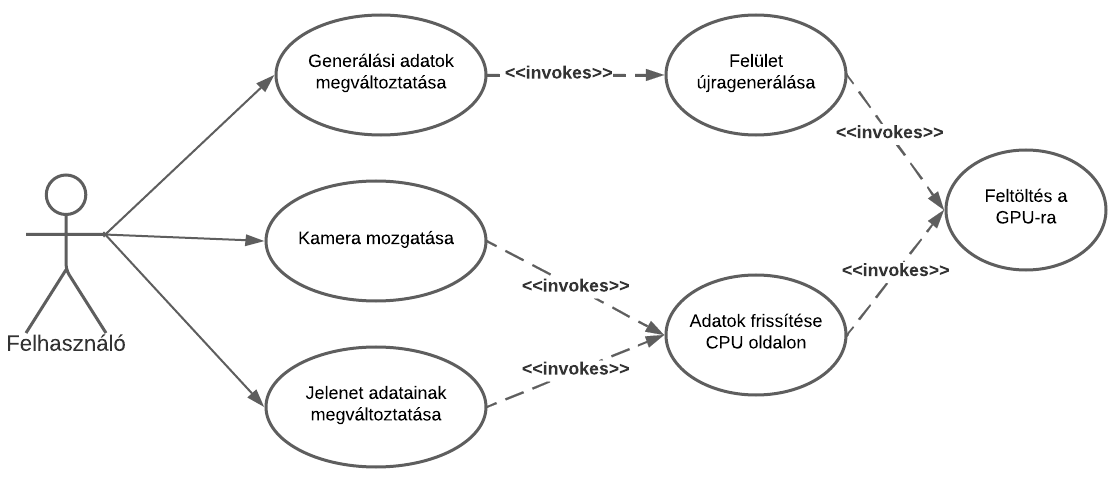
\includegraphics[width=0.8\textwidth]{usecase.png}
	\caption{Felhasználói eset diagram}
	\label{fig:usecase}
\end{figure}

% ------------------------------------------------------
%\chapter{Implementáció}
%\label{ch:impl}
% ------------------------------------------------------

\section{Implementáció}

Ebben a részben néhány fontos implementációs részletre térek ki. Ennek motivációja, hogy a CPU implementáció profilozásakor kiderült, az algoritmus az idő $60\%$-át a felület kiértékelésével és a gradiens kiszámításával tölti.

\section{de Casteljau-algoritmus}
\subsection{Iterációval}
Az algoritmus CPU implementációja két egymásba ágyazott ciklussal működik. Ez \aref{lst:iter}-es forráskódban látható.

\begin{lstlisting}[caption={de Casteljau iterációval}, language={C++}, label={lst:iter}]
	float deCasteljou_iter(float4 pts, float t, float one_minus_t)
	{
		for (int j = 1; j <= 3; j++)
		{
			for (int i = 0; i <= 3 - j; i++)
			{
				pts[i] = one_minus_t * pts[i] + t * pts[i + 1];
			}
		}
		return pts[0];
	}
\end{lstlisting}

\subsection{Swizzle operátorokkal}
Részben azért esett a választás a köbös Bézier-felületekre, mert a GPU kód támogat műveleteket legfeljebb $4$ elemű vektorokkal. Ez azt jelenti, hogy a felület kontrollponthálójának egy sora belefér egy ilyen vektorba. Az elméleti áttekintésnél láttuk, hogy a felület kiértékelése visszavezethető az egydimenziós problémára, így ezt a függvényt kell vektorizálni. Ezt a szintén hardveresen támogatott ún. swizzle operátorokkal tesszük. Ezek lényege, hogy a művelet elvégzése előtt a bemeneti vektorok elemeit tetszőlegesen átrendezhetjük, akár duplikálhatjuk is. A javított implementáció \aref{lst:swizzle}-es forráskódban látható.

\begin{lstlisting}[caption={de Casteljau swizzle operátorokkal}, language={C++}, label={lst:swizzle}]
	float deCasteljou_swizzle(float4 pts, float t, float one_minus_t)
	{
		for (int j = 1; j <= 3; j++)
		{
			pts.xyz = one_minus_t * pts.xyz + t * pts.yzw;
		}
		return pts[0];
	}
\end{lstlisting}

A programokat először a Radeon GPU Analyzer-rel hasonlítottam össze. A gépi kódban már egyáltalán nem lesz ciklus, mert a driver kibontja. A ciklusos implementációban 11, a swizzle implementációban 10 vektorművelet szerepelt. Ebből messzemenő következtetést nehéz levonni. A swizzle implementáció ciklusát kézzel is kibontottam. Ez nem okozott jelentős javulást. Végül lecseréltem minden sort egy lerp (lineáris interpoláció) utasításra. Az implementáció \aref{lst:lerp}-as forráskódban látható. Ezt a driver jobban tudja optimalizálni. 

\lstset{}
\begin{lstlisting}[caption={de Casteljau lerp függvénnyel}, language={C++}, label={lst:lerp}]
	float deCasteljou_lerp(float4 pts, float t)
	{
		pts.xyz = lerp(pts.xyz, pts.yzw, t);
		pts.xy = lerp(pts.xy, pts.yz, t);
		return lerp(pts.x, pts.y, t);
	}
\end{lstlisting}


\subsection{Mérési eredmények}
Az algoritmusokat a ,,Brute force'' távolságmező-generáló módszer segítségével hasonlítottam össze, mert ez főként felületkiértékelést végez. Minden esetben egy $32^3$ méretű textúrát generáltam és kiátlagoltam $512$ futtatást. \Aref{tab:deCasteljau} és \ref{tab:deCasteljau2} táblázatok a számításhoz szükséges GPU-időt foglalják össze milliszekundumban. Először a Bézier-felületből készített magasságtérképet textúrába írtam, majd a távolságmező generálásakor onnan kiolvastam. \Aref{tab:deCasteljau} táblázat második oszlopában ezek az értékek szerepelnek. A harmadik oszlopban a távolságmező generálásakor számítottam ki a függvényértékeket.

Referenciának kimockoltam a de Casteljau-függvényt azzal, hogy csak az utolsó sort hagytam meg. A GPU Analyzer-ből kiderül, hogy ekkor teljesen eltűnik a függvény, mert a driver mindenhol inline-olja. Ezt az értéket kivontam a harmadik oszlopból, így megkaptam, mekkora része a futási időnek a felület kiértékelése.

\begin{table}[H]
	\begin{center}
		\begin{tabular}{| c || c || c | c |}
			\hline
			(ms) & \textbf{Memóriából olvasva} & \textbf{Számítva} & \textbf{ebből de Casteljau} \\ 
			\hline\hline
			két ciklusos & 51,6 & 76,97	& 75,76 \\
			\hline
			swizzle	& 51,35	& 2,74 & 1,53 \\
			\hline
			kibontott & 51,33 & \textbf{2,63} & 1,42 \\
			\hline
			üres & 51,41 & 1,21	& 0 \\
			\hline
		\end{tabular}
	\end{center}
	\caption{de Casteljau-algoritmus mérése egy $32^3$ méretű textúrán}
	\label{tab:deCasteljau}
\end{table}

A mérésekből kiderül, hogy a ciklusos implementáció nagyjából \emph{50-szer lassabb} GPU-n, mint a többi számításos verzió. A második oszlopban az értékek nagyjából megegyeznek, a futási idők pedig jóval a táblázatban szereplő legjobb idő felett vannak. Ebből arra következtethetünk, hogyha memóriából olvassuk ki a felületértékeket, akkor a limitáció a memóriaelérés által okozott késleltetés lesz.

A legjobb megoldásokat összehasonlítottam egy nagyobb, $64^3$ méretű textúrán is. Ennek eredményeit \aref{tab:deCasteljau2} táblázat tartalmazza.

\begin{table}[H]
	\begin{center}
		\begin{tabular}{| c || c || c | c |}
			\hline
			(ms) & \textbf{Számítva} & \textbf{ebből de Casteljau} \\ 
			\hline\hline
			swizzle & 64,09 & 49,38 \\
			\hline
			kibontott & 62,13 & 47,42 \\
			\hline
			lerp & \textbf{52,85} & 38,14 \\
			\hline
			üres & 14,71 & 0 \\
			\hline
		\end{tabular}
	\end{center}
	\caption{de Casteljau-algoritmus mérése egy $64^3$ méretű textúrán}
	\label{tab:deCasteljau2}
\end{table}

A kézzel kibontott ciklus nem okoz lényeges javulást, viszont a lineáris interpoláció nagyjából $25\%$-kal gyorsabb. 


\subsection{Megjegyzések}
\begin{itemize}
	\item A felület kiértékeléséhez a kontrollpontháló minden sorára meg kell hívni az algoritmust, majd az eredményekből álló vektorra megint. Ehhez összesen ötször kell meghívni a de Casteljau-függvényt.
	\item Matematikailag létezik ennél gyorsabb algoritmus, de nem használjuk, mert a numerikus stabilitásra nagyon oda kell figyelni GPU környezetben. (Szűk számábrázolás miatt.)
	\item Emellett az is megfigyelhető, hogy a matematikai műveletigény és a driver által generált kód futási ideje között nem feltétlenül intuitív az összefüggés.
\end{itemize}


\section{Pont-felület távolság és gradiense}

\subsection{Analitikus pont-felület távolság}
Legyen $E(e_1,e_2,e_3)$ a mintavételezési pont modellkoordináta-rendszerben és $r(x,y) = (x,y,b(x,y))$ pedig a felület parametrikus egyenlete. Ekkor a távolság egy adott felületi és mintavételezési pontra:
$$ D_1(x,y) = \norm{E-r}_2 = \sqrt{(e_1-x)^2 + (e_2-y)^2 + (e_3-b(x,y))^2} $$
Ennek egyik parciális deriváltja: 
$$ \partial_xD_1 = \frac{2(x-e_1) + 2(b(x,y)-e_3)b_x(x,y)}{\sqrt{(e_1-x)^2 + (e_2-y)^2 + (e_3-b(x,y))^2}} $$
Ahol $b_x(x,y)$ a magasságfüggvény $x$ szerinti parciális deriváltja. A nevezőben lévő érték a távolság, ami a felület közelében $0$ közeli. Mivel a távolségfüggvényt a felülethez közel is kiértékeljük, ez mindenképp numerikusan instabil lesz, sőt, nullával osztást is eredményezhet. 

A távolságfüggvényhez a legközelebbi pontot akarjuk meghatározni a felületen. Mivel a négyzetgyök függvény szigorúan monoton nő, a norma négyzetének is ugyanott lesz minimum helye, ahol a normának.
$$ D(x,y) = \norm{E-r}_2^2 = (e_1-x)^2 + (e_2-y)^2 + (e_3-b(x,y))^2 $$
Ennek parciális deriváltjai: 
$$ \partial_xD = 2(x-e_1) + 2(b(x,y)-e_3)b_x(x,y) $$
$$ \partial_yD = 2(y-e_2) + 2(b(x,y)-e_3)b_y(x,y) $$
Ezt sokkal könnyebben és stabilabban tudjuk számolni.

\subsection{Gradiens számításának műveletigénye}
Távolságfüggvényeknél gyakori, hogy a gradienst a szimmetrikus differencia módszerrel határozzuk meg. Ehhez nem kell ismerni a távolságfüggvény képletét, csak ki kell értékelni több helyen. Egy kis $\varepsilon$ számot választva a gradiens közelítése: 
$$ b' \approx \frac{1}{2\varepsilon} \cdot \begin{pmatrix} b(x+\varepsilon,y) - b(x-\varepsilon,y) \\ b(x,y+\varepsilon) - b(x,y-\varepsilon) \end{pmatrix} $$
Itt a $b(x,y)$ függvény kiértékelését négyszer el kell végezni. Emellett egy kivonásra és egy szorzásra is szükség van. ($1/(2\varepsilon)$ konstans) Ez összesen 122 matematikai művelet. 

A parciális derivált számításához csak 12 mátrix elemet kell redukálni, így annak kiértékelése 22 matematikai művelet. $b$ totális deriváltjának analitikus számításához a két parciális deriváltat kell kiszámolni, ami 44 művelet. Mivel az utóbbi matematikailag hatékonyabb, ezt a verziót implementáltam.

\subsection{A távolság gradiense}
A totális derivált kifejezhető vektorokkal:
$$ D' = 2\left[\left(\begin{pmatrix} x \\ y \end{pmatrix} - \begin{pmatrix} e_1 \\ e_2  \end{pmatrix}\right)  + (b(x,y)-e_3)\cdot b'(x,y) \right]$$
Ezt a gradienst használjuk az iterációs módszerben. 


\section{AdaMax}
A AdaMax algoritmus kódja a pszeudokóddal teljesen ekvivalens. Kizárólag a numerikus stabilitásra kell figyelni. A vetített gradiens számításánál az $\varepsilon$ érték nem lehet túl kicsi. $\varepsilon = 10^{-6}$ érték például már a végeredményben is látható numerikus hibákat okoz. Én $\varepsilon = 10^{-4}$ értéket használtam.

Szintén numerikus hibák és a zéróosztás elkerülése végett a tapasztalati szórás minimumát is $10^{-4}$-re állítottam. Ez alapján $u$ frissítési szabálya: 
$$ u_t = \max (\beta_2 u_{t-1}, |g_t|, 10^{-4}) $$

\section{A program tesztelése}

A program célja ugyanazon felület megjelenítése több különböző módszerrel. A módszerek listája: 
\begin{itemize}
	\item Háromszögekkel tesszellált felület megjelenítése raszterizációval
	\item Felületgenerálás Lipschitz-módszerrel, majd sugárkövetés
	\item Felületgenerálás Brute Force módszerrel, majd sugárkövetés
	\item Felületgenerálás AdaMax módszerrel, majd sugárkövetés
\end{itemize}
A tesztek eredménye, hogy a felület minden esetben helyesen jelenik meg. Ha a felületet a raszterizációval egyidejűleg rajzoljuk ki, azt is megállapíthatjuk, hogy a mélységértékek is helyesek. Ez lehetővé teszi, hogy a felületet más objektumokkal egyidejűleg rajzoljuk ki.


\section{Keretrendszer és egyéb függőségek}

A programomat a Falcor \cite{Kallweit22} grafikus keretrendszer 5.2-es verziójában készítettem el. A Falcor verziók visszafelé általában nem kompatibilisek, így mindenképpen ezt a verziót kell használni. A függőségeket főként a keretrendszer szabja meg ezek közül a legfontosabbak:

\begin{itemize}
	\item Windows 10
	\item Visual Studio 2019
	\item Windows 10 SDK
	\item GPU és DirectX 12 Driver
\end{itemize}

A keretrendszer a CMake build rendszert használja.

\section{Projekt összeállítása és fordítás}

A projekt összeállításának lépései:
\begin{itemize}
	\item A Falcor grafikus keretrendszer letöltése: \codeword{git clone https://github.com/NVIDIAGameWorks/Falcor.git} majd visszaállítás 5.2-es verzióra: \codeword{git reset --hard 430824f0}
	\item Kód elhelyezése a \codeword{Falcor\Source\Samples\SDFBox\} mappában
	\item A mappa hozzáadása a CMake build rendszerhez \codeword{add_subdirectory(SDFBox)}
	\item A projekt létrehozása a \codeword{setup_vs2019.bat} szkript futtatásával
	\item A projekt a \codeword{build/windows-vs2019-d3d12} mappába kerül, melyet Visual Studio 2019-el lehet megnyitni.
	\item A teljes solution-t nem érdemes lefordítani elegendő az \codeword{SDFBox} projekt lefordítása.
	\item A program a \codeword{build\windows-vs2019-d3d12\bin\Release\} mappából futtatható.
\end{itemize}




\cleardoublepage

% ------------------------------------------------------
\chapter{Eredmények}
% ------------------------------------------------------

Az alábbi mérési eredményeket ugyanazon tesztpéldákon végeztem el mindhárom módszerre. A használt videókártya egy Nvidia GTX 1060 Ti notebook GPU. A felbontás minden esetben Full HD.

\begin{figure}[H]
	\centering
	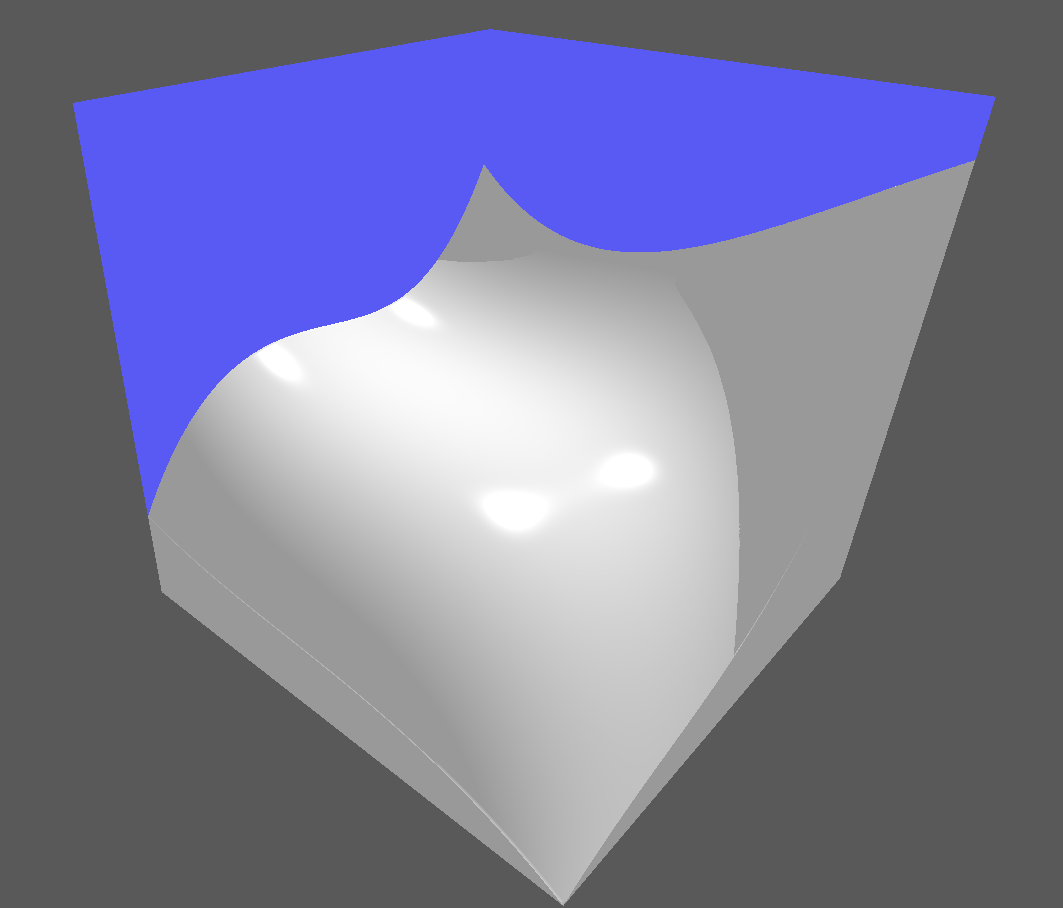
\includegraphics[width=0.5\textwidth]{result.png}
	\caption{Bézier-felület}
	\label{img:bezSurf}
\end{figure}

\section{Generálási módszer hatása a sugárkövetésre}

Itt azt hasonlítom össze, hogyan hat a sphere trace algoritmus futási idejére a generálási módszer. \Aref{tab:trace} táblázat utolsó oszlopa 512 képkocka megjelenítésének átlagos GPU-idejét foglalja össze. A jelenetben minden esetben egy véletlenszerűen generált Bézier-felület és egy pontfényforrás szerepelt, amihez ún. kemény árnyékokat számítottam.

\begin{table}[H]
	\begin{center}
		\begin{tabular}{| c || c | c |}
			\hline
			\textbf{Generálási módszer} & \textbf{Szükséges lépésszám} & \textbf{Átlagos GPU idő (ms)} \\ 
			\hline\hline
			Lipschitz & $512<$ & 1,47 \\
			\hline
			Brute force & $<256$ & 0,95 \\
			\hline
			Adam & $<256$ & 0,96 \\
			\hline
		\end{tabular}
	\end{center}
	\caption{Generálási módszer hatása a sugárkövetésre}
	\label{tab:trace}
\end{table}

\subsection{Lipschitz-módszer}
A Lipschitz-módszer időköltsége a memóriaigénnyel egyenesen arányos. Az ilyen algoritmusok minden esetben memórialimitáltak. A generált távolságmező olyan rossz minőségű, hogy alacsony látószögből még 512 lépésben sem konvergál a sugárkövetés. A generálás emellett olyan olcsó, hogy akár sugárkövetéskor, a pixel shaderben is kiszámítható. Ezt a módszert a következőkben nem tárgyalom.

\subsection{Brute Force módszer}
A Brute Force módszer meglehetősen költséges, azonban a generált távolságmező (a rácspontokban) biztosan optimális, így 256 iteráció minden esetben elég volt.

\subsection{AdaMax módszer}
A tesztek meglepő eredménye, hogy az AdaMax algoritmusban 25-nél nagyobb iterációszám egy esetben sem javított a képminőségen. Ennek egyik oka, hogy a felület közelében a 10. pont miatt nagyon gyorsan konvergál a módszer. Másik oka, hogy ha a sugárkövetés során beleszaladunk a felületbe egy rossz becslés miatt, akkor a következő távolságkiértékelés negatív lesz, és visszatalálunk a felülethez. A sugárkövetéshez továbbra is elegendő volt 256 iteráció minden esetben, így kijelenthetjük, hogy a szimulációs eredményeket sikerült megerősíteni.


\section{Távolságmező-generálás}
Mivel a Lipschitz-módszer csak egy gyenge alsó közelítést ad a távolságmezőre, így a Brute Force algoritmust hasonlítottam össze az AdaMax algoritmust használó  módszerrel. \Aref{tab:gen} táblázatban az előbb bemutatott tesztpélda távolságmezőjének generálásához szükséges átlagos GPU-idők szerepelnek a felbontás függvényében, milliszekundumban.

\begin{table}[H]
	\begin{center}
		\begin{tabular}{| c || c | c | c | c | c | c | c | c |}
			\hline
			\textbf{Felbontás} & 16	& 32 & 48 & 64 & 80 & 96 & 112 & 128 \\ 
			\hline\hline
			\textbf{Brute force} & 0.17 & 2.18 & 16.87 & 52.23 & 185.79 & 382.57 & - & - \\
			\hline
			\textbf{AdaMax} & 1.09 & 4.36 & 15.82 & 28.04 & 63.49 & 92.65 & 163.07 & 219.13
			\\
			\hline
		\end{tabular}
	\end{center}
	\caption{A generálás ideje a felbontás függvényében, milliszekundumban}
	\label{tab:gen}
\end{table}

Az értékeket \aref{img:bf-adam} grafikonon meg is jelenítettem:

\begin{figure}[H]
	\centering
	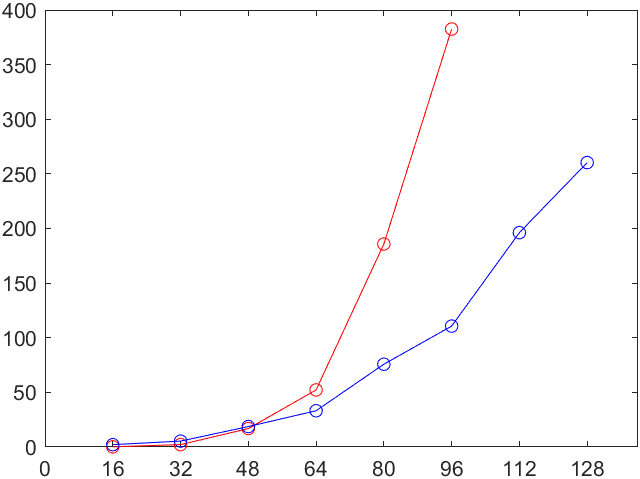
\includegraphics[width=0.4\textwidth]{bf-adam.png}
	\caption{A generálás ideje a felbontás függvényében, milliszekundumban}
	\label{img:bf-adam}
\end{figure}

\Aref{tab:gen} teszt eredményeiből látszik, hogy a két módszer algoritmikus komplexitásából adódó különbségek már kis felbontás esetén ($64^3$) is jelentősek. A komplexitásbeli különbség oka, hogy amíg a Brute Force megoldás a függvényt egyre növekvő felbontáson értékeli ki, addig az új módszer fix lépést végez 10 pontból.

\section{Összehasonlítás a tesszellációval}
A felületet a sugárkövetés mellett háromszögekkel közelítve is megjeleníthetjük. A két módszer eltéréseit úgy tudjuk vizualizálni, ha sugárkövetés után a fragment shaderben beleírjuk a mélység adatot a mélység bufferbe, és az egyik felület árnyalását valami egyszerűre cseréljük. \Aref{img:zfight} ábrán  a sugárkövetett felületet Blinn--Phong-árnyalással, a háromszögekkel tesszelláltat pedig egy egyszerű színskálával jelenítettem meg.

\begin{figure}[H]
	\centering
	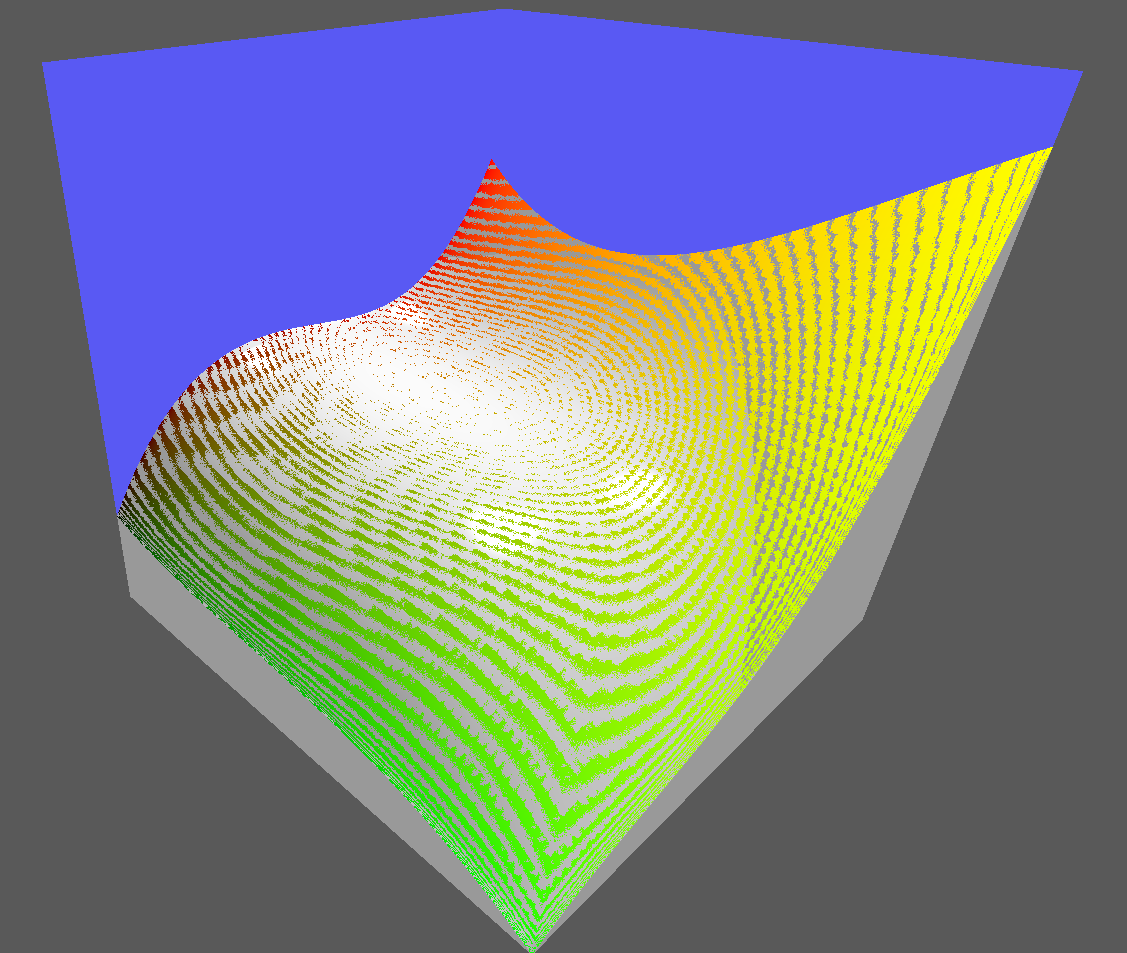
\includegraphics[width=0.4\textwidth]{zfight.png}
	\caption{Tesszellált és sugárkövetett felület egyszerre kirajzolva}
	\label{img:zfight}
\end{figure}

\Aref{img:zfight} ábrán a két módszerrel kirajzolt felület színe váltakozva jelenik meg. Ennek oka, hogyha a mélységbuffer értékei helyesek, akkor átlátszatlan felületeknél minden pixel színe a legközelebbi felület színe lesz. A váltakozás oka, hogy amíg felületet tartalmazó voxelekben a sugárkövetés egy bilineáris felületet határoz meg, addig a raszterizációnál a felületet két, a csúcspontokban interpoláló háromszöggel közelítjük.

A raszterizációt felhasználhatjuk arra, hogy az első sugárkövetést megspóroljuk és csak az árnyékokhoz használjunk sugárkövetést. Ezt a technikát használják például az Unreal Engine-ben is puha árnyékok számításásra. \cite{RayTracedDistanceFieldShadowing} \Aref{tab:rast} táblázatban egy, az előzőektől független teszt eredményei láthatók. A második oszlopba egy képkocka kirajzolásához szükséges átlagos GPU-idő került.

\begin{table}[H]
	\begin{center}
		\begin{tabular}{| c || c | c |}
			\hline
			\textbf{Generálási módszer} & \textbf{Átlagos GPU idő (ms)} \\ 
			\hline\hline
			Lipschitz & 0,72 \\
			\hline
			Brute force & 0,51 \\
			\hline
			AdaMax & 0,50 \\
			\hline
			Háromszögelés + AdaMax & 0,24 \\
			\hline
		\end{tabular}
	\end{center}
	\caption{Sugárkövetés helyettesítése raszterizációval}
	\label{tab:rast}
\end{table}





% ------------------------------------------------------
\chapter{Összefoglalás}
\label{ch:sum}
% ------------------------------------------------------

A dolgozatomban bemutattam és implementáltam a távolságmezők generálásának alapvető módszereit, majd áttekintettem a parametrikus- és Bézier-felületek elméleti hátterét. Fő eredményként bemutattam, hogyan használhatók gradiens módszerek távolságmezők generálásához, és szimulációval validáltam az AdaMax algoritmus alkalmazhatóságát köbös Bézier felületek távolságmezőjének generálására. Kitértem a módszer GPU-implementációjának részleteire, mellyel nagyságrendekkel gyorsítottam a kiértékelést. Végül mérésekkel igazoltam, hogy az új módszer már kis felbontáson is lényegesen gyorsabb, mint a referencia implementáció.

\cleardoublepage

% Acknowledgements (optional) - in case your thesis received funding or would like to express special thanks to someone
\chapter*{\acklabel}
\addcontentsline{toc}{chapter}{\acklabel}
Köszönet illeti a témavezetőmet, Bán Róbertet az elméleti háttér és a program  kidolgozásában nyújtott segítségéért.

A Kulturális és Innovációs Minisztérium ÚNKP-22-6 kódszámú Új Nemzeti Kiválóság Programjának a Nemzeti Kutatási, Fejlesztési és Innovációs Alapból finanszírozott szakmai támogatásával készült.

% Appendices (optional) - useful for detailed information in long tables, many and/or large figures, etc.
%\appendix
%\input{samples_hu/sim.tex}
%\cleardoublepage

% Bibliography (mandatory)
\phantomsection
\addcontentsline{toc}{chapter}{\biblabel}
\printbibliography[title=\biblabel]
\cleardoublepage

% List of figures (optional) - useful over 3-5 figures
\phantomsection
\addcontentsline{toc}{chapter}{\lstfigurelabel}
\listoffigures
\cleardoublepage

% List of tables (optional) - useful over 3-5 tables
%\phantomsection
%\addcontentsline{toc}{chapter}{\lsttablelabel}
%\listoftables
%\cleardoublepage

% List of algorithms (optional) - useful over 3-5 algorithms
%\phantomsection
%\addcontentsline{toc}{chapter}{\lstalgorithmlabel}
%\listofalgorithms
%\cleardoublepage

% List of codes (optional) - useful over 3-5 code samples
%\phantomsection
%\addcontentsline{toc}{chapter}{\lstcodelabel}
%\lstlistoflistings
%\cleardoublepage

% List of symbols (optional)
%\printnomenclature

\end{document}
